\documentclass[preprint,12pt]{elsarticle}

\usepackage{amsmath,amssymb,amsthm}
\usepackage[ruled,linesnumbered]{algorithm2e}
\theoremstyle{definition}
\newtheorem{theorem}{Theorem}
\newtheorem{proposition}[theorem]{Proposition}
\newtheorem{corollary}[theorem]{Corollary}
\newtheorem{lemma}[theorem]{Lemma}
\newtheorem{definition}{Definition}
\newtheorem{remark}{Remark}
\newtheorem{assumption}{Assumption}
\usepackage{booktabs}
\usepackage{array}
\usepackage{threeparttable}
\usepackage{graphicx}
\usepackage{float}
\usepackage{hyperref}
\hypersetup{hidelinks}
\usepackage{setspace}
\usepackage[nopatch=footnote]{microtype}
\usepackage{pdflscape}
\usepackage{adjustbox}

\graphicspath{{ProvidedFigures/}{Charts/}}

\journal{}

\raggedbottom
\clubpenalty=10000
\widowpenalty=10000
\displaywidowpenalty=10000
\interfootnotelinepenalty=10000
\setlength{\emergencystretch}{2em}

% Float packing: let LaTeX place multiple figures per page instead of one-per-page.
\setcounter{topnumber}{3}
\setcounter{bottomnumber}{2}
\setcounter{totalnumber}{4}
\renewcommand{\topfraction}{0.94}
\renewcommand{\bottomfraction}{0.85}
\renewcommand{\textfraction}{0.06}
\renewcommand{\floatpagefraction}{0.72}

\makeatletter
\renewcommand{\footnoterule}{%
  \kern -3pt
  \hrule width .4\columnwidth
  \kern 2.6pt
}
\makeatother

\begin{document}

\begin{frontmatter}

\title{Structure-Preserving Randomization Inference for Decision Timing}

\author{Aryan Patel}
\ead{ampatel355@gmail.com}
\address{Independent Researcher}

\begin{abstract}
\begingroup
\parindent=0pt
\emergencystretch=3em
A realized return does not identify skill: profit confounds the quality of a
decision sequence, the structural exposure it implies, and the drift of the path on
which it ran. We develop \emph{structure-preserving randomization inference}, a
conditional randomization test that isolates the contribution of decisions by holding
the realized structure and exogenous path fixed and re-randomizing only the decision
margin from a chosen conditional law. We treat the choice of conditioning measure as
model risk: each verdict is point-identified only given a measure, so the data return a
sensitivity range over a declared menu, with a valid intersection--union test for the
measure-invariant claim, whose power is set by the least-favorable measure. The test is
finite-sample valid conditional on the chosen law and, under a stated central-limit
condition, consistent in the trade count $N$ at rate $N^{-1/2}$ against a per-trade
location-shift alternative; against a pure-exposure alternative it carries zero
noncentrality. Correspondingly, in a controlled structural-exposure world White's
Reality Check and Hansen's SPA (single-strategy specialization) reject a
profitable-but-untimed strategy about two-thirds of the time, while the placement test
holds its nominal size of $0.050$. Applied to daily gold futures, no strategy in an
eleven-rule panel rejects under the neutral measure, and across $322$ cross-asset tests
nothing survives multiplicity control; four volatility-filtered rules reject under
volatility-state-matched measures, locating the residual signal at the state-conditioning
margin, but no robust, measure-invariant entry-timing skill survives. The construction
applies wherever a decision sequence is overlaid on an exogenous process, subject to a
feasibility and exchangeability check.
\endgroup
\end{abstract}

\begin{keyword}
conditional randomization inference \sep model risk \sep uncertainty quantification \sep
Monte Carlo methods \sep sensitivity analysis \sep backtesting \sep data snooping \sep reproducibility
\end{keyword}

\vspace{2pt}
\noindent\emph{JEL Classification:} C12; C15; C58; G14. \quad
\emph{MSC 2020:} 62F03; 62G09; 91G70.

\end{frontmatter}

\section{Introduction}

A realized return does not identify skill. When a decision rule is run on a single
price path and turns a profit, that profit confounds at least three things: the
quality of the decisions, the structural exposure those decisions imply, and the
drift of the path itself. To separate them we need a counterfactual, but not just any
counterfactual. The comparison that matters is an implementation that carries the
\emph{same} structural burden on the \emph{same} path and differs only in the margin
whose value is in question. Without it, profitability and exposure are not
separately identified. A backtest then remains a description rather than a test.

This paper develops a procedure for that comparison, which we call
\emph{structure-preserving randomization inference}. The idea is a conditional
randomization test in the sense of Fisher \cite{Fisher1935} and Cand\`es et al.\
\cite{Candes2018}: we fix the realized structure and re-randomize only the object of
interest, drawing it from a known conditional law. Concretely, when a decision sequence is overlaid
on an exogenous process, the realized data induce a \emph{structure} (the geometry of
the sequence) and a placement of that geometry. Holding the structure and the process
fixed while randomizing placement isolates the decisions' marginal contribution. We
randomize the placement and not the path because it is the placement, not the path,
whose value is in question, and the validity of the comparison rests on the
exchangeability of placements under the conditioning law, not on any model for the
process. The construction is indexed by a family of
structure-preserving measures $\mathbb{Q}=\{\mathbb{Q}_\theta:\theta\in\Theta\}$, all
fixing the structure and the path but differing in which additional features of the
realized arrangement they hold fixed; each $\mathbb{Q}_\theta$ defines a sharp null
$H_0^\theta$ and an estimand $q_\theta=\mathbb{Q}_\theta\big(T(S)\ge T(S_0)\big)$, where
$T$ is the statistic and $S_0$ the realized placement. Which features count as
``structure'' and which as ``the decision'' is the analyst's modeling choice,
and making that choice explicit is what separates a stated null from an informal
benchmark. Because the choice is not pinned down by the data, the procedure reports
the verdict's dependence on it as a sensitivity range across a declared admissible
menu of measures, which we read as the model risk the choice of null induces. The
contribution is thus methodological.

The leading application, and the one we develop in full, is the entry-timing skill of a
trading strategy. Here the structure is the realized trade geometry (the price path,
trade count, holding-period multiset, inter-trade-gap multiset, capital weights, and
direction sequence), and the object randomized is the placement of trades on the
calendar. The test asks a narrow, falsifiable question: conditional on its realized
structural burden, does a strategy's entry placement earn more than a structurally
matched random implementation would earn on the same path? A strategy then exhibits
entry-placement skill only when its realized timing beats that counterfactual, not
merely when it is profitable. The empirical testbed is daily gold futures (GC=F) over
2002-03-04 to 2026-04-02, an asset whose buy-and-hold cumulative return of $14.670$ over
the window makes the confound between drift and timing especially stark.

Three properties distinguish the procedure from a study of any one asset. First,
the test is a finite-sample valid conditional randomization test (Theorem
\ref{prop:q-validity}): under $H_0^\theta$ the realized placement is exchangeable with
its $\mathbb{Q}_\theta$-draws, so the Monte Carlo tail area is super-uniform at every
level, with the standardized conditional excess $\mathrm{RCSI}_z$ retained only as a
descriptive, approximately pivotal effect size. Second, the measure family supports a
sensitivity-analysis theory of timing skill across a declared menu of measures
(Section~\ref{sec:theory}). Because the
measures differ exactly in where they draw the line between structure and placement, a
rejection under one but not another is confounded with the conditioning choice, which
the data do not pin down; we therefore identify \emph{measure-invariant} entry-placement
skill as rejection of $H_0^\theta$ for every $\theta$ in an admissible class, and we
characterize the test's local power (one-sided Gaussian power
$\beta(h)=\Phi(h-z_{1-\alpha})$ along the Pitman sequence $\zeta_N=h/\sqrt N$, with a
minimum detectable edge that shrinks at the $N^{-1/2}$ rate) and its orthogonality:
against a pure structural-exposure alternative the test carries noncentrality zero, by
construction. Third, that orthogonality is shown head-to-head against return-based
tests. On known-truth worlds (Section~\ref{sec:competitor}), White's Reality Check
\cite{white2000} and Hansen's SPA \cite{hansen2005}, tests of profitability rather than
placement, reject a profitable-but-untimed strategy about two-thirds of the time
(rejection rates $0.660$ and $0.638$), while the structure-preserving null holds its
nominal size ($0.050$). The single-strategy specialization of these return tests is a
degenerate use of White's and Hansen's procedures: they answer a different question
(profitability, not placement), and on a profitable-but-untimed strategy that
difference is what separates the verdicts.

The paper's \emph{primary contribution} is the procedure: the conditional randomization
test, its finite-sample validity, and the sensitivity-range theory of the measure
family. The remaining results are \emph{secondary}, included to make the procedure
usable rather than
to stand alone. A calibration-and-power study, comprising five synthetic worlds with known ground
truth and a positive control on the real GC=F path
(Section~\ref{sec:simulation-validation}), shows the
test is correctly sized and that its power rises with signal quality; the head-to-head
competitor comparison locates where return-based inference fails; and a
cross-asset panel of $322$ strategy-by-asset evaluations across $47$ instruments
(Section~\ref{sec:cross-asset-multiplicity}) applies the test at breadth under joint
multiplicity control. Applied to the GC=F panel, no strategy rejects at $p\le0.05$ before
or after Benjamini--Hochberg adjustment, and the verdict is robust to a leading-gap
feasibility restriction but sensitive to two state-preserving measures, context-matched and regime-preserving
(Section~\ref{sec:schedule-sensitivity}), which is exactly the measure-dependence the
theory formalizes, made empirical. The substantive reading is not that the
strategies are bad, but that within the scope of the timing test, realized profitability
is often not separately identifiable from structural exposure. The powered, seed-robust
evidence is single-asset (gold); the $322$-test cross-asset panel is an availability
sample and the multi-asset and frequency checks are exploratory, so the empirical role
here is to demonstrate the method rather than to make a broad market claim.

\section{Related literature}

\paragraph{Data snooping and backtest overfitting.} The literature on strategy
evaluation is largely a literature on multiplicity. White's Reality Check
\cite{white2000}, Hansen's SPA test \cite{hansen2005}, and the universe-search framing of
Sullivan, Timmermann, and White \cite{sullivan1999} control the error of selecting the
best rule \emph{across} a universe of candidates; the backtest-overfitting program
\cite{bailey2017,baileylopez2014,lopezdeprado2018} and the factor-zoo critique of
Harvey, Liu, and Zhu \cite{harveyliuzhu2016} extend the same warning to research degrees
of freedom and the resulting inflation of discoveries. These procedures take each
strategy's realized decision sequence as given and ask whether the \emph{best} of many is
genuinely good. Our object is orthogonal and within-strategy: holding the realized trade
geometry and price path fixed, we ask whether a single rule's entry \emph{placement}
carries information. The two layers are complementary (the between-strategy correction
bounds selection risk, the conditional test isolates timing), and we run the panel under
both.

\paragraph{Resampling of returns.} Bootstrap methods for dependent data (the stationary
bootstrap of Politis and Romano \cite{politisromano1994} and the moving-block bootstrap of
K\"unsch \cite{Kunsch1989}) preserve the statistical properties of the \emph{return
series} and resample it to quantify uncertainty in profitability under a generic
return-generating process. By construction they perturb the path. The structure-preserving
test does the opposite: it holds the realized path fixed and randomizes only placement, so
it inherits the market's autocorrelation, fat tails, volatility clustering, and regime
dynamics without a return model, and answers a timing question that a path-perturbing
resample cannot pose. Section~\ref{sec:competitor} reports that
return-based tests reject a profitable-but-untimed strategy where the placement test holds
size.

\paragraph{Conditional and Fisher randomization inference.} The procedure is a conditional
randomization test. Its validity derives, in the tradition of Fisher \cite{Fisher1935}
and the exact permutation and invariance theory of Lehmann and Romano \cite{LehmannRomano2005},
from a known re-randomization of the realized data rather than a postulated population
model; Ernst \cite{Ernst2004} surveys this exactness and Pesarin and Salmaso
\cite{PesarinSalmaso2010} treat permutation tests that preserve rich dependence rather
than assuming i.i.d.\ data. The specific posture, conditioning on a structure and resampling only
the object of interest from a known conditional law, is the conditional randomization
construction of Cand\`es et al.\ \cite{Candes2018}. What is new here is the conditioning
set: the realized trade geometry of a strategy, which makes the relevant exchangeability
an exchangeability of \emph{schedules} rather than of \emph{returns}, in the sense of
Aldous \cite{Aldous1985}. Imposing a known re-randomization on data that were not produced by a designed experiment is the program of randomization inference in observational settings, developed at length by Rosenbaum \cite{Rosenbaum2002}, where the reported object is a range of verdicts traced out as a modeling assumption is varied; our sensitivity range across the admissible menu $\Theta_0$ is a device of the same kind, with the conditioning measure in the role Rosenbaum's bias parameter plays. The argument is also design-based in the finite-population sense of Imbens and Rubin \cite{ImbensRubin2015}: the realized price path and structural profile are held fixed and only the placement is randomized, though here the resampled object is a constrained schedule rather than a treatment assignment and the target is a tail probability rather than an average effect. The same exchangeability engine underwrites conformal prediction \cite{Vovk2005,Lei2018}, a sibling paradigm that converts it into finite-sample coverage for prediction sets rather than into a level for a hypothesis test; we borrow nothing operationally from it and note the connection only to place the construction within the broader family of distribution-free, exchangeability-based procedures.

\paragraph{Selective and post-selection inference.} By defining a test conditional on the
structure a strategy actually produced, the method controls a \emph{selective} type-I
error in the sense of Fithian, Sun, and Taylor \cite{FithianSunTaylor2014}: validity is
recovered by characterizing the law of the statistic conditional on the realized selection
event, the same posture as exact post-selection inference \cite{LeeSunSunTaylor2016}. This
deliberately differs from the simultaneous-over-all-selections guarantee of Berk et al.\
\cite{BerkBrownBujaZhangZhao2013}: we condition on the realized structure rather than
protect against every structure that might have been chosen. The measure family makes the
conditioning event itself the modeling object, so that what is held fixed, and therefore
what skill is identified against, is stated explicitly rather than left implicit.

\paragraph{Multiple-testing control.} Applied at breadth across a $322$-test panel,
inference is corrected jointly. We report Benjamini--Hochberg \cite{benjaminihochberg1995}
false-discovery-rate control and the $q$-value perspective of Storey \cite{Storey2002},
the stepwise data-snooping procedure of Romano and Wolf \cite{romanowolf2005}, and the
Benjamini--Yekutieli \cite{BenjaminiYekutieli2001} guarantee that holds under the positive
and, conservatively, arbitrary dependence that correlated assets and overlapping strategy
logic induce.

\paragraph{Efficiency and adaptive markets.} The economic backdrop is the long debate over
whether persistent abnormal performance is extractable from price data. Efficiency
arguments emphasize its difficulty \cite{fama1970}; the adaptive-markets view allows for
episodic, regime-dependent opportunity \cite{lo2004}; and evidence on time-series momentum
documents directional effects in some asset classes while robust inference remains hard
\cite{moskowitz2012}. We take no stance on this debate. The procedure provides a
conditional test: a way to ask, for any one strategy on any one path, whether its timing
adds value beyond the exposure it carries.


\section{Methodology}

A trading strategy maps market information to a sequence of exposure decisions;
its realized return is the product of an exogenous return process and an
endogenous timing process. A backtest reports that product, and it is often read as
skill, though it fuses the quality of entry placement, the structural
exposure the strategy's geometry implies, and the drift of the realized path. We
isolate the first. Conditional on the realized structural profile, the test asks
whether entry placement earns more than a structure-matched random implementation
on the same path.

\begin{definition}[Structure-preserving null and entry-placement skill]
Let $\{P_t\}_{t=0}^{T}$ be a realized price path. The \emph{structural profile} of a strategy is the tuple $\mathcal{S} = (\mathbf{h}, \mathbf{g}^{\mathrm{int}}, g^{\mathrm{ext}}, \boldsymbol{\omega}, \mathbf{d})$ consisting of the realized holding-duration multiset $\mathbf{h}$, the internal gap multiset $\mathbf{g}^{\mathrm{int}}$, the external slack $g^{\mathrm{ext}}$, the capital weights $\boldsymbol{\omega}$, and the direction signs $\mathbf{d}$. A \emph{feasible schedule} is any placement of the trade sequence on the open-price calendar that preserves $\mathcal{S}$ and admits no overlapping positions. The structure-preserving null is the distribution $\mathbb{Q}$ over feasible schedules induced by Algorithm~\ref{alg:spr} below. A strategy is said to exhibit \emph{entry-placement skill} at level $\alpha$ if its realized return $CR^{\mathrm{actual}}$ exceeds the $(1-\alpha)$ quantile of $CR^{\mathrm{sim}}$ under $\mathbb{Q}$.
\end{definition}

Entry-placement skill is, then, the excess of realized return over what the strategy's structural footprint would produce under randomized placement. It is a deliberately narrow object, tested against a sharp counterfactual, and we do not claim it exhausts the colloquial meaning of skill.

\subsection{Formal problem statement}

Let strategy $s$ produce a realized cumulative return $CR_s^{\mathrm{actual}}$ from a trade sequence $\mathcal{T}_s$ applied to the observed price path $\{P_t\}_{t=0}^{T}$. The inferential question is whether $CR_s^{\mathrm{actual}}$ reflects favorable entry placement after conditioning on the realized structural profile, or whether it is consistent with the returns achievable by a structurally identical strategy whose entry points are randomly placed on the same price path.

The structure-preserving null hypothesis and its alternative are defined as follows:
\begin{quote}
$H_0$: The realized entry schedule of strategy $s$ is exchangeable with random timing under $\mathbb{Q}$, conditional on the strategy's structural constraints (trade count, holding durations, inter-trade gaps, direction, and capital allocation) and the observed price path. Under $H_0$, the strategy's entry points contain no information beyond what is embedded in its structural burden.

\medskip

$H_1$: The realized entry schedule of strategy $s$ produces returns that systematically exceed those achievable under random timing with the same structural constraints. Under $H_1$, the entry points reflect incremental entry-placement information.
\end{quote}

The test is one-sided because the claim under evaluation is that a strategy's entry placement is \emph{better} than chance, not merely different from chance. The null distribution is generated by the structure-preserving Monte Carlo procedure described in Section~\ref{sec:spr}, and rejection of $H_0$ at significance level $\alpha$ constitutes evidence of entry-placement skill at that confidence level.

\subsection{Data, execution, and trade extraction}

The data pipeline (feature construction and forward-safe regime labeling), the next-bar execution and fill model, and the eleven strategy rules are specified in the Online Supplement (Section~S1); all strategies share next-bar execution, non-overlapping positions, and an expected round-trip cost $c=0.000470$ applied identically to the realized trades and to every simulated schedule. Because the null preserves the trade count and sizing and reprices on the same path, the per-trade cost (and any roll-induced distortion embedded in the continuous GC=F series, which is held fixed under $\mathbb{Q}$) enters the realized and randomized schedules in the same way and largely differences out of the placement contrast; randomized placement changes the prices and capital base at which the rate is levied, so the cancellation is approximate rather than exact, and any frictions not re-applied to the simulated schedules would, if anything, ease the null's competitors and bias the test toward non-rejection. The verdict is thus conservative with respect to cost specification; the Online Supplement (Section~S2) confirms detection is unchanged with stochastic execution costs enabled on the high-signal positive control, though a panel-wide scan of the near-threshold strategies under stochastic costs remains to be run, and the buy-and-hold benchmark below ($14.670$, a gross $\sim$15.7$\times$ multiple over $2002$--$2026$, cost-free and inclusive of roll) is reported only to scale the asset's drift, not as a tradeable comparator. We retain here only the trade-structure objects the null requires.

For each strategy \(s\), let the realized trade sequence be
\begin{equation}
\mathcal{T}_s=\{(\tau^{\mathrm{in}}_j,\tau^{\mathrm{out}}_j,\omega_j,d_j)\}_{j=1}^{N_s},
\end{equation}
where \(\tau^{\mathrm{in}}_j\) and \(\tau^{\mathrm{out}}_j\) are the realized entry and exit timestamps, \(\omega_j\) is the realized fraction of portfolio value allocated to the position at entry, and \(d_j\) is the direction sign. In the reported panel, all strategies are long-only, so \(d_j=+1\) for every trade.

Trade times are mapped onto the observed open-price calendar. If \(i^{\mathrm{in}}_j\) and \(i^{\mathrm{out}}_j\) denote the corresponding calendar indices, the realized holding duration is
\begin{equation}
h_j=i^{\mathrm{out}}_j-i^{\mathrm{in}}_j.
\end{equation}
Any non-positive duration is ruled out. If a recorded holding length disagrees with the duration implied by the saved entry and exit timestamps, the timestamp-implied duration is used.

The null model also preserves the strategy's spacing pattern. For consecutive trades, the realized internal gap is
\begin{equation}
g^{\mathrm{int}}_j=i^{\mathrm{in}}_{j+1}-i^{\mathrm{out}}_j,\qquad j=1,\ldots,N_s-1.
\end{equation}
The total external slack is the sum of the leading slack before the first trade and the trailing slack after the last trade,
\begin{equation}
g^{\mathrm{ext}} = i^{\mathrm{in}}_1 + \left(I_{\max}-i^{\mathrm{out}}_{N_s}\right),
\end{equation}
where \(I_{\max}\) is the final open-price index in the sample. A transition indicator is also retained for each pair of consecutive trades: it equals 0 if the next trade begins on the same bar as the previous exit and 1 otherwise. Overlapping realized trades are not permitted.

\subsection{Conditioning set and estimand}
\label{sec:conditioning-estimand}

The conditioning set for strategy $s$ is
\[
\mathcal{C}_s =
\sigma\!\left(
\{P_t\}_{t=0}^{T},
N_s,
\mathbf{h},
\mathbf{g}^{\mathrm{int}},
g^{\mathrm{ext}},
\boldsymbol{\omega},
\mathbf{d},
\mathcal{A}_s
\right),
\]
where $\mathcal{A}_s$ denotes the open-price calendar and non-overlap feasibility constraints induced by the realized trade log. Conditional on $\mathcal{C}_s$, the only object randomized is the calendar placement of the realized trade template. The test therefore does not ask whether the entire strategy is skilled. It asks whether the realized entry schedule is unusually favorable after the realized duration, spacing, sizing, direction, and price-path information have already been absorbed into $\mathcal{C}_s$.

Let $\mathcal{F}(\mathcal{C}_s)$ be the feasible schedule space consistent with $\mathcal{C}_s$, and let $S_0\in \mathcal{F}(\mathcal{C}_s)$ be the realized schedule. For any schedule $S$, let $T(S)$ be the cumulative return obtained by applying the preserved weights, directions, and holding durations to the observed open-price path. The estimand is the conditional entry-placement advantage
\[
\Delta_Q(s)=T(S_0)-\mathbb{E}_{S\sim \mathbb{Q}}\!\left[T(S)\mid \mathcal{C}_s\right],
\]
together with the upper-tail probability
\[
p_Q(s)=\mathbb{Q}\!\left(T(S)\ge T(S_0)\mid \mathcal{C}_s\right).
\]
The reported RCSI estimates $\Delta_Q(s)$ using the simulated mean, while the Monte Carlo $p$-value estimates $p_Q(s)$ using finite draws from $\mathbb{Q}$. These are conditional quantities tied to the chosen schedule distribution $\mathbb{Q}$; they are not unconditional estimates of total trading ability.

\subsection{Structure-preserving randomization}
\label{sec:spr}

The reported results use a structure-preserving random-timing null. In plain terms: each simulation keeps every trade's duration, size, and direction exactly as the strategy generated them, but randomly shifts \emph{when} those trades occur on the calendar. Concretely, (i) we randomly choose how much idle time precedes the first trade and (ii) we randomly reorder the gaps between consecutive trades. Holding periods and the price path are untouched. The strategy's structural footprint is preserved; only its calendar placement is replaced with a random alternative consistent with that footprint.

Formally, the null holds fixed the observed market path, the realized trade count, each trade's holding duration, each trade's fraction of capital at risk, the long-only direction sequence, and the realized spacing burden between trades. Only the placement of the trade sequence on the observed calendar is randomized.

Let \(\mathbf{h}=(h_1,\ldots,h_{N_s})\) denote the realized duration vector and let \(\mathbf{g}^{\mathrm{int}}\) denote the realized internal-gap vector. For each simulation, a leading gap is drawn uniformly from the feasible range,
\begin{equation}
g^{\mathrm{lead}} \sim \mathrm{DiscreteUniform}\{0,\ldots,g^{\mathrm{ext}}\},
\end{equation}
the realized internal gaps are randomly permuted, and the randomized entry indices are generated recursively as
\begin{equation}
\tilde{i}^{\mathrm{in}}_1=g^{\mathrm{lead}}, \qquad
\tilde{i}^{\mathrm{in}}_{j+1}=\tilde{i}^{\mathrm{in}}_j+h_j+\tilde{g}^{\mathrm{int}}_j,
\end{equation}
with randomized exits
\begin{equation}
\tilde{i}^{\mathrm{out}}_j=\tilde{i}^{\mathrm{in}}_j+h_j.
\end{equation}
This construction preserves the exact duration profile and the multiset of realized internal gaps rather than only their averages. Because all realized gaps are non-negative and the final exit must remain within the available calendar, simulated trades cannot overlap and every simulated schedule is feasible by construction. Same-bar rotations are preserved whenever they occur in the realized strategy, because zero-gap transitions remain zero under permutation.

No additional state matching beyond these structural constraints is imposed in the reported runs. Algorithm~\ref{alg:spr} states the procedure in step-by-step form.

\begin{algorithm}[H]
\caption{Structure-preserving randomization of a single trade schedule}
\label{alg:spr}
\KwIn{Realized durations $\mathbf{h}=(h_1,\ldots,h_{N_s})$; realized internal gaps $\mathbf{g}^{\mathrm{int}}=(g^{\mathrm{int}}_1,\ldots,g^{\mathrm{int}}_{N_s-1})$; external slack $g^{\mathrm{ext}}$; price calendar of length $I_{\max}+1$.}
\KwOut{Randomized entry indices $(\tilde{i}^{\mathrm{in}}_1,\ldots,\tilde{i}^{\mathrm{in}}_{N_s})$ and exit indices $(\tilde{i}^{\mathrm{out}}_1,\ldots,\tilde{i}^{\mathrm{out}}_{N_s})$ with no overlapping trades.}
Draw $g^{\mathrm{lead}}\sim\mathrm{DiscreteUniform}\{0,\ldots,g^{\mathrm{ext}}\}$\;
Draw a uniformly random permutation $\pi$ of $\{1,\ldots,N_s-1\}$ and set $\tilde{g}^{\mathrm{int}}_j=g^{\mathrm{int}}_{\pi(j)}$\;
Set $\tilde{i}^{\mathrm{in}}_1\leftarrow g^{\mathrm{lead}}$ and $\tilde{i}^{\mathrm{out}}_1\leftarrow \tilde{i}^{\mathrm{in}}_1+h_1$\;
\For{$j\leftarrow 2$ \KwTo $N_s$}{
$\tilde{i}^{\mathrm{in}}_j\leftarrow \tilde{i}^{\mathrm{out}}_{j-1}+\tilde{g}^{\mathrm{int}}_{j-1}$\;
$\tilde{i}^{\mathrm{out}}_j\leftarrow \tilde{i}^{\mathrm{in}}_j+h_j$\;
}
\Return $(\tilde{i}^{\mathrm{in}},\tilde{i}^{\mathrm{out}})$
\end{algorithm}

\paragraph{Sampling distribution.} Algorithm~\ref{alg:spr} samples from a distribution $\mathbb{Q}$ over feasible schedules: the marginal of $g^{\mathrm{lead}}$ is uniform on $\{0,\ldots,g^{\mathrm{ext}}\}$ and the marginal of $\tilde{\mathbf{g}}^{\mathrm{int}}$ is uniform over the permutations of $\mathbf{g}^{\mathrm{int}}$. $\mathbb{Q}$ is not the uniform measure over all non-overlapping schedules consistent with $\mathcal{S}$ (that measure is combinatorially expensive to construct when gaps differ in size), but it preserves the realized spacing multiset exactly and is invariant under relabeling of trade indices. The reported $p$-value is a one-sided permutation $p$-value under $H_0:\,CR^{\mathrm{actual}}\stackrel{d}{=}CR^{\mathrm{sim}}\mid \mathcal{S}, \{P_t\},\,\text{schedule}\sim\mathbb{Q}$, with the plus-one Monte Carlo correction $(1+k)/(M+1)$; its level is exact in the limit $M\to\infty$ when the realized timing is exchangeable with $\mathbb{Q}$ under $H_0$, and a Monte Carlo approximation in finite samples.

\begin{definition}[No-entry-skill null]
\label{def:h0}
Fix the realized price path $\{P_t\}$ and structural profile $\mathcal{S}$. The \emph{no-entry-skill null} $H_0$ is the hypothesis that the realized schedule $S_0$ is itself a draw from $\mathbb{Q}$; equivalently, that $S_0,S_1,\ldots,S_M$ are exchangeable conditional on $(\mathcal{S},\{P_t\})$. Entry-placement skill is, by construction, a violation of $H_0$: realized timing that is favorably non-exchangeable with $\mathbb{Q}$. The theorem below is therefore a statement about this defined null, not an assumption that any particular strategy satisfies it.
\end{definition}

\subsection{The measure family}

The choice of $\mathbb{Q}$ is part of the null hypothesis, not a theorem forced by the data. A robust empirical conclusion should therefore be checked against nearby schedule measures. Table~\ref{tab:schedule_measures} lists the main alternatives and the interpretation each would support.

\begin{table}[H]
\centering
\caption{Schedule distributions for sensitivity analysis.}
\label{tab:schedule_measures}
\small
\renewcommand{\arraystretch}{1.12}
\begin{tabular}{@{}>{\raggedright\arraybackslash}p{0.26\textwidth}>{\raggedright\arraybackslash}p{0.34\textwidth}>{\raggedright\arraybackslash}p{0.30\textwidth}@{}}
\toprule
Schedule measure & Preserved features & Interpretation \\
\midrule
Gap-permutation $\mathbb{Q}$ used here & Price path, ordered durations, gap multiset, weights, directions, non-overlap & Entry placement conditional on realized spacing burden \\
Uniform feasible schedules & Price path, durations, weights, directions, non-overlap & Entry placement under a less restrictive spacing null \\
Slack-redistribution schedules & Price path, durations, weights, directions, approximate turnover & Sensitivity to exact preservation of realized gaps \\
Context-matched schedules & Price path, durations, weights, directions, and coarse entry context such as volatility or day-of-week & Incremental entry skill beyond simple market-state matching \\
Block or regime-preserving schedules & Price path, durations, weights, directions, and regime occupancy constraints & Timing conditional on staying within comparable market regimes \\
\bottomrule
\end{tabular}
\end{table}

The primary GC=F results use the gap-permutation measure, with robustness checked in Section~\ref{sec:schedule-sensitivity}, which re-evaluates the full panel under a context-matched measure, a leading-gap feasibility restriction, and a regime-preserving robustness measure. The reported admissible menu $\Theta_0$ comprises the gap-permutation, leading-gap, and context-matched measures; the regime-preserving measure is reported alongside them as a second volatility-state replication check, a coarser forward-safe discretization of the same state, and the uniform-feasible and slack-redistribution variants are listed as candidates and left to future work. As anticipated here, the verdict turns out to be null-sensitive across measures, which is why we treat agreement across schedule measures, not rejection under any single one, as the standard for a robust timing claim.

\paragraph{Conservatism of the conditioning set.} The holding-period multiset $\mathbf{h}$ and the internal-gap multiset $\mathbf{g}^{\mathrm{int}}$ are themselves outputs of the strategy's decision rule, not exogenous primitives. Conditioning on them attributes any predictive content embedded in exit logic, holding-period selection, and turnover regulation to the structural profile rather than to the entry-placement test. This is a deliberate, conservative design choice: a strategy whose edge resides in adaptive exits, in selectively skipping trades, or in volatility-scaled holding periods will not reject the null even when those decisions are genuinely informative. Non-rejection is therefore silence about the conditioned dimensions rather than a floor on skill: rejection is strong evidence of edge in entry placement, but non-rejection is consistent with skill residing in the conditioned dimensions or in their interaction with placement (Section~\ref{sec:limitations}).

\subsection{Conditional excess return and its standardized form}

The two reported effect-size measures are standard conditional contrasts, not new statistics; we name them only for brevity and notational economy. Let \(CR_s^{\mathrm{actual}}\) denote the realized cumulative return of strategy \(s\), and let \(\{CR_{s,m}^{\mathrm{sim}}\}_{m=1}^{M}\) denote the simulated cumulative returns under the structure-preserving null, with sample mean \(\mu_s^{\mathrm{sim}}\) and standard deviation \(\sigma_s^{\mathrm{sim}}\). The \emph{conditional excess return} is the realized return net of the null mean,
\begin{equation}
\mathrm{RCSI}_s = CR_s^{\mathrm{actual}} - \mu_s^{\mathrm{sim}},
\end{equation}
and its \emph{standardized} form is the Monte Carlo $z$-score,
\begin{equation}
\mathrm{RCSI}_{z,s}=\frac{CR_s^{\mathrm{actual}}-\mu_s^{\mathrm{sim}}}{\sigma_s^{\mathrm{sim}}}.
\end{equation}
The first is the effect size on the return scale; the second is that effect in null-standard-deviation units and, by the argument of Section~\ref{sec:theory}, is asymptotically pivotal under $\mathbb{Q}$. Neither carries the verdict on its own: classification rests on the exact $p$-value and percentile, with the standardized excess reported only as a descriptive effect size. When the null standard deviation is zero, $\mathrm{RCSI}_z$ is set to zero if the realized return equals the null mean and is otherwise undefined.

The one-sided empirical \(p\)-value is computed using the smoothed estimator
\begin{equation}
\hat{p}_s
=
\frac{1+\sum_{m=1}^{M}\mathbf{1}\{CR_{s,m}^{\mathrm{sim}}\ge CR_s^{\mathrm{actual}}\}}{M+1},
\end{equation}
and the realized percentile rank is
\begin{equation}
\pi_s
=
100\times
\frac{1+\sum_{m=1}^{M}\mathbf{1}\{CR_{s,m}^{\mathrm{sim}}\le CR_s^{\mathrm{actual}}\}}{M+1}.
\end{equation}
The analysis also reports \(p\)-value prominence, defined as \(-\log_{10}(p)\), together with the 5th and 95th simulated percentiles for distributional context. These quantities jointly measure whether the realized timing of a strategy is unusually favorable relative to random timing under the same structural burden.

\begin{assumption}[Standing assumptions]
\label{ass:standing}
The reported procedure rests on the following, collected here once so that
they need not be inferred from the construction. We separate the conditions
the test's \emph{validity} requires from those invoked only for the
\emph{asymptotic} statements of Section~\ref{sec:theory}. We do not assume any
model for returns.

\medskip
\noindent\emph{Validity conditions.}

\begin{description}
\item[(A1) Exchangeability under the reference law.] Conditional on the
$\sigma$-field $\mathcal C_s=\sigma(\{P_t\}_{t=0}^{T},\allowbreak N_s,\allowbreak\mathbf h,
\allowbreak\mathbf g^{\mathrm{int}},\allowbreak g^{\mathrm{ext}},\allowbreak\boldsymbol\omega,\allowbreak\mathbf d,
\allowbreak\mathcal A_s)$ of Section~\ref{sec:conditioning-estimand}, the null
$H_0^\theta$ is the hypothesis that the realized schedule $S_0$ is
exchangeable with i.i.d.\ draws $S_1,\dots,S_M\sim\mathbb{Q}_\theta$; this
holds in particular when $S_0\stackrel{d}{=}\mathbb{Q}_\theta$ given
$\mathcal C_s$. Every level statement is conditional on $\mathcal C_s$ and on
this exchangeability alone. \emph{Used by} the finite-sample validity result
(Theorem~\ref{prop:q-validity}(i)) and, through it, the orthogonality and
intersection--union results (Theorems~\ref{prop:orthogonality},
\ref{prop:iut}).

\item[(A2) Conditioning content.] The conditioning information is exactly
$\mathcal C_s$ above, with $\mathcal A_s$ the open-price calendar and its
non-overlap feasibility constraints. The structural profile
$\mathcal S=(\mathbf h,\mathbf g^{\mathrm{int}},g^{\mathrm{ext}},
\boldsymbol\omega,\mathbf d)$ and the price path $\{P_t\}$ are held fixed and
treated as exogenous to the test, even though the holding-duration multiset
$\mathbf h$ and the internal-gap multiset $\mathbf g^{\mathrm{int}}$ are
themselves outputs of the strategy. Any predictive content embedded in exit
logic, holding-period selection, or turnover is therefore attributed to
$\mathcal S$, not to placement, and every reported quantity is conditional on
this partition; a different defensible partition defines a different null
(Section~\ref{sec:measure-family}). \emph{Used by} the definition of the
estimand and every standardization in Section~\ref{sec:theory}; it is what
Proposition~\ref{prop:nonsuff} reasons about.

\item[(A3) Feasibility and strict non-overlap.] All realized internal gaps
are non-negative and the realized template fits the calendar, so the recursion
of Algorithm~\ref{alg:spr} returns only non-overlapping schedules whose final
exit lies at or before $I_{\max}$. The support of $\mathbb{Q}_\theta$ is exactly
this feasible set; zero-gap (same-bar) transitions are preserved because they
remain zero under permutation. \emph{Used by} the support of the reference law
and Lemma~\ref{lem:admissible-validity}.

\item[(A4) Reference law.] The primary reference law $\mathbb{Q}$ is the
gap-permutation measure: the leading gap is drawn
$g^{\mathrm{lead}}\sim\mathrm{DiscreteUniform}\{0,\dots,g^{\mathrm{ext}}\}$ and
the internal-gap vector is set to a uniformly random permutation of the
realized $\mathbf g^{\mathrm{int}}$. This law preserves the realized spacing
multiset exactly, is invariant to relabeling of trade indices, and is
\emph{not} the uniform measure over feasible schedules. $\mathbb{Q}$ is an
analyst's choice and is part of $H_0$, not a consequence forced by the data;
robustness is therefore reported as a sensitivity range over the admissible
menu $\Theta_0$ (Section~\ref{sec:measure-family}), with $\mathbb{Q}$ the
minimum element $\mathbb{Q}_{\mathrm{gp}}$. \emph{Used by} the construction of
$\mu_{\mathbb Q}$, $\sigma_{\mathbb Q}$, and $q_\theta$, hence every $p$-value,
percentile, and effect size.

\item[(A5) Monte Carlo approximation.] The reported $p$-value is the plus-one
estimator $\hat p_M=(1+k)/(M+1)$ with $M$ finite ($M=5{,}000$ throughout). Its
level is exact on the attainable $p$-grid in the limit $M\to\infty$ under (A1),
and a Monte Carlo approximation at finite $M$; the $+1$ in numerator and
denominator guarantees validity and rules out an invalidly-zero $p$-value. For
\emph{any} fixed $S_0$, $\hat p_M\to q_\theta$ almost surely. \emph{Used by}
Theorem~\ref{prop:q-validity}.

\item[(A6) One-sidedness.] The test is one-sided: it asks whether the realized
placement is \emph{favorably} non-exchangeable with $\mathbb{Q}_\theta$. All
$p$-values are upper-tail, all power functions are one-sided
($\beta(h)=\Phi(h-z_{1-\alpha})$), and the intersection--union test maximizes
one-sided per-measure $p$-values. \emph{Used by} Corollary~\ref{prop:local-power}
and Theorem~\ref{prop:iut}.

\item[(A7) Direction.] The reported panel is long-only ($d_j=+1$ for every
trade); the direction vector $\mathbf d$ is part of the conditioned structural
profile and is held fixed under $\mathbb{Q}_\theta$, not randomized. The
framework permits a general $\mathbf d$, but the empirical claims and the
noncentrality signs of Section~\ref{sec:theory} are stated under $\mathbf d=+1$.

\item[(A8) Approximate cost cancellation.] The expected round-trip cost
$c=0.000470$ is applied identically to the realized and to every simulated
schedule. Because randomized placement changes the prices and the capital base
at which the rate is levied, this cancellation is approximate, not exact; any
frictions not re-applied to the simulated schedules would only ease the null's
competitors and bias the test toward non-rejection, so the verdict is
conservative with respect to cost specification. Detection is confirmed
unchanged under stochastic execution costs in the Online Supplement
(Section~S2).
\end{description}

\medskip
\noindent\emph{Asymptotic conditions (used in Section~\ref{sec:theory}; not
needed for validity).} The following are invoked only by the consistency,
minimum-detectable-edge, and local-power statements; the test's level rests on
(A1) alone, and $\mathrm{RCSI}_z$ is reported as an approximately pivotal
effect size under these conditions, not as a basis for the verdict.

\begin{description}
\item[(A9) Finite calendar; large-$N$ regime.] The calendar has finite length
$I_{\max}+1$ and the template has a finite trade count $N$, so the resampling
orbit is finite. At small $N$ the placement margin is weakly identified, only $(N-1)!$ internal-gap
arrangements carry spacing information and the minimum detectable edge is large, so such
cases (for instance Squeeze Breakout with $N=4$) are read as exploratory rather than
inferential.
Asymptotic statements are taken as $N\to\infty$ along a sequence of structurally
comparable fixed-path templates, evidence accumulating in $N$ rather than in
the length of the price path.

\item[(A10) Weak ($\alpha$-mixing) dependence.] The realized path is
$\alpha$-mixing, so its autocorrelation decays fast enough to be absorbed into
the finite-population permutation variance rather than break the normal
approximation. This is part~(b) of Assumption~\ref{ass:clt}; it is cross-listed
here for visibility and is not restated.

\item[(A11) No-dominant-term (Lindeberg-type) condition.]
$\max_j\mathrm{Var}(\xi_j)/\allowbreak\sum_j\mathrm{Var}(\xi_j)\to0$, so that no single
trade carries a non-negligible share of the return budget and the variance
accumulates linearly, $\sigma_{\mathbb Q}\asymp\sqrt N\,\sigma_1$. This is
part~(a) of Assumption~\ref{ass:clt}; it is cross-listed here for visibility and
is not restated. We do not claim to have verified it for the gold path: the
condition is sufficient, not necessary, and is falsifiable, failing precisely
when one or a few trades dominate the return budget.

\item[(A12) Alternative-law normality.] Under the per-trade location-shift
alternative of Theorem~\ref{prop:consistency} the centered statistic
$Z_N-\delta_N\to_d N(0,1)$, with $\delta_N$ the deterministic displacement defined
there, so the location shift moves the limit law without altering its Gaussian
shape. This is the final clause of Assumption~\ref{ass:clt}, cross-listed here for
visibility and not restated; it is what licenses the residual-normality step in the
consistency and local-power proofs.
\end{description}
\end{assumption}

\section{Theoretical properties}
\label{sec:theory}

This section collects the formal properties of the test. We establish its
finite-sample validity (Theorem~\ref{prop:q-validity}); a named central-limit
condition (Assumption~\ref{ass:clt}) and the consistency, detection-rate, and
local-power results that follow from it (Theorem~\ref{prop:consistency},
Corollary~\ref{prop:local-power}); the orthogonality of the test to exposure
(Theorem~\ref{prop:orthogonality}); and, because the conditioning measure is a
declared modeling choice, the treatment of the timing estimand as a sensitivity
range over a declared admissible menu of measures, for whose boundary
(measure-invariant skill) we give a valid intersection--union test
(Theorem~\ref{prop:iut}). Throughout, $T(S)$ is the cumulative-return statistic
induced by a schedule $S$, $S_0$ is the realized schedule, and
$\mathcal C=\sigma(\mathcal S,\{P_t\})$ is the conditioning $\sigma$-field of
Section~\ref{sec:conditioning-estimand}. Longer proofs are deferred to
\ref{app:proofs}.

\subsection{Finite-sample validity}
\label{sec:fs-validity}

The validity of the procedure rests on no model for returns, but on the
analyst's choice of reference law $\mathbb{Q}_\theta$: it requires only that the
realized statistic be exchangeable with its resampled counterparts under that
chosen law. We restate the result at the level of the statistic, so that the
section is self-contained and the conditions are visible. Validity is therefore
\emph{exact against the sharp null} $H_0^\theta$: it is a property of the test
relative to a target of inference fixed by the analyst, not a property the
procedure can claim independently of which conditioning law is declared.

\begin{theorem}[Finite-sample validity and large-$M$ consistency of the
Monte Carlo $p$-value]
\label{prop:q-validity}
Fix any structure-preserving measure $\mathbb{Q}_\theta$ in the family
$\mathfrak Q$ of Definition~\ref{def:measure-family}, and let $S_1,\dots,S_M$ be
i.i.d.\ draws from $\mathbb{Q}_\theta$ given $\mathcal C$.
Define
\[
\hat p_M
=\frac{1+\sum_{m=1}^{M}\mathbf 1\{T(S_m)\ge T(S_0)\}}{M+1}.
\]
\emph{(i) Validity.} Suppose $H_0^\theta$ holds in the statistic-level form that
$T(S_0)$ is exchangeable with $\{T(S_m)\}_{m=1}^{M}$ given $\mathcal C$; this
holds in particular if $S_0\stackrel{d}{=}\mathbb{Q}_\theta$ given $\mathcal C$.
Then $\hat p_M$ is super-uniform: for every $\alpha$ on the grid
$\{1/(M+1),\dots,1\}$, $\Pr(\hat p_M\le\alpha\mid\mathcal C)\le\alpha$, with
equality absent ties and strict conservatism when ties are counted into the
right tail.
\emph{(ii) Consistency in $M$.} For \emph{any} fixed $S_0$, whether or not
$H_0^\theta$ holds, $\hat p_M\to q_\theta:=\mathbb{Q}_\theta\big(T(S)\ge
T(S_0)\mid\mathcal C\big)$ almost surely as $M\to\infty$.
\end{theorem}

\begin{proof}
(i) Exchangeability of $T(S_0)$ with $\{T(S_m)\}_{m=1}^{M}$ given $\mathcal C$
makes the rank of $T(S_0)$ among $\{T(S_m)\}_{m=0}^{M}$ uniform on
$\{1,\dots,M+1\}$ absent ties; this holds whenever $S_0\stackrel{d}{=}
\mathbb{Q}_\theta$ given $\mathcal C$, because then $S_0,S_1,\dots,S_M$ are
themselves exchangeable and $T$ is a fixed measurable map. Dividing the
upper-tail rank by $M+1$ and counting ties into the right tail gives
$\Pr(\hat p_M\le\alpha\mid\mathcal C)\le\alpha$; ties only enlarge the numerator
of $\hat p_M$, so they move the bound strictly toward conservatism and can never
inflate the rejection probability. (ii) For fixed $S_0$ the indicators
$\mathbf 1\{T(S_m)\ge T(S_0)\}$, $m\ge1$, are i.i.d.\ Bernoulli$(q_\theta)$
given $\mathcal C$; the strong law of large numbers yields the limit, which does
not invoke $H_0^\theta$.
\end{proof}

Part~(i) is the finite-sample validity of a Monte Carlo randomization test:
drawing $M$ schedules rather than enumerating $\mathbb{Q}_\theta$ preserves exact
level-$\alpha$ validity \cite{Dwass1957,Hope1968}; the modern group-theoretic
account is \cite{HemerikGoeman2018}, and the $+1$ in numerator and denominator is
what makes $\hat p_M$ valid at finite $M$: the naive $\sum\mathbf
1\{\cdot\}/M$ is downward biased and can be invalidly zero
\cite{PhipsonSmyth2010}. Because the null is generated by a constrained,
dependence-preserving resampling of one realized path rather than by i.i.d.\
draws, the relevant guarantee is that of \cite{BesagClifford1989}, which is exact
for precisely this conditional-on-the-data construction. The guarantee is exact
against $H_0^\theta$: $\mathbb{Q}_\theta$ is an analyst-chosen object, and the
property transfers only insofar as the realized schedule is exchangeable with its
$\mathbb{Q}_\theta$-resamples under $H_0^\theta$, and only on the attainable
$p$-grid. Two distinct granularities should not be conflated. The first is
intrinsic to the orbit. When $N$ is small the placement information is carried by only
the $(N-1)!$ internal-gap permutations, while the leading-gap draw mainly relocates the
whole template in calendar time, an exposure channel rather than a spacing channel, so
the placement margin is weakly identified, with the large minimum detectable edge of
Theorem~\ref{prop:consistency}. The orbit itself need not be coarse: exact enumeration
of the $N=4$ Squeeze Breakout orbit gives $6\times471=2{,}826$ feasible schedules with
$2{,}826$ distinct statistic values and an exact one-sided tail probability of $0.057$
under the deterministic-cost gap-permutation null (Online Supplement, Section~S3), short
of significance and consistent with the Monte Carlo $p=0.053$. Near-threshold small-$N$
verdicts are therefore read as exploratory because the placement margin is weakly
identified, not because the $p$-grid is coarse. The second granularity is
the Monte Carlo budget $M$, which only refines the grid the orbit already admits:
the dependence of the rejection probability on $M$ is nonmonotone, in that on each
plateau where $k_\alpha=\lfloor\alpha(M+1)\rfloor-1$ is constant the rejection
probability declines, jumping upward only when $\alpha(M+1)$ crosses an integer,
so the finite-$M$ power traces a sawtooth around its $M\to\infty$ limit
\cite{Hope1968}; at $M=5{,}000$ and $\alpha=0.05$ this budget is far from binding.
In both cases the consequence is a loss of power, never a
loss of size: small $N$ is an identification and power problem, not a validity problem,
because Theorem~\ref{prop:q-validity}(i) bounds the conditional rejection
probability by $\alpha$ on the whole attainable grid.

\subsection{A central-limit condition for the standardized statistic}
\label{sec:clt-assumption}

The consistency, minimum-detectable-edge, and local-power results below are
asymptotic, and they require a limit theorem for the standardized statistic. We
do not have an i.i.d.\ structure to invoke: under $\mathbb{Q}_\theta$ the trade
contributions are a gap-permutation of one fixed, autocorrelated return path, so
the summands are neither independent nor identically distributed, and the
placements are further coupled by the non-overlap constraint and the shared path.
We therefore state the needed Gaussian approximation as an explicit, named
high-level condition and prove the propositions \emph{conditional} on it, rather
than assert it as a by-product.

\begin{assumption}[Combinatorial / finite-population CLT condition]
\label{ass:clt}
Write $\log(1+CR)=\sum_{j=1}^{N}\xi_j$, where under $\mathbb{Q}_\theta$ the $\xi_j$
are the $N$ trade log-contributions evaluated at a placement of the fixed
duration/gap template drawn from $\mathbb{Q}_\theta$ on the fixed path. Let
$\mu_{\mathbb Q},\sigma_{\mathbb Q}$ denote the conditional $\mathbb{Q}_\theta$
mean and standard deviation of $T(S)=\log(1+CR)$ and set
$Z_N=(T(S_0)-\mu_{\mathbb Q})/\sigma_{\mathbb Q}$. We assume that under
$H_0^\theta$,
\[
Z_N \;\to_d\; N(0,1) \qquad (N\to\infty),
\]
and that this convergence holds under the following two regularity requirements:
\emph{(a)} a no-dominant-term, Lindeberg-type condition
$\max_{j}\mathrm{Var}(\xi_j)/\allowbreak\sum_{j}\mathrm{Var}(\xi_j)\to0$, so that no
single trade carries a non-negligible share of the return budget; and
\emph{(b)} weak ($\alpha$-mixing) dependence of the realized path, so that the
autocorrelation entering the permutation variance decays fast enough for the
finite-population variance to be the correct standardization. We further assume
that under the per-trade location-shift alternative of
Theorem~\ref{prop:consistency} the centered statistic $Z_N-\delta_N\to_d N(0,1)$,
with $\delta_N$ the deterministic displacement defined there, so that the
location shift moves the limit law without altering its Gaussian shape.
\end{assumption}

Assumption~\ref{ass:clt} is a high-level condition, not a corollary of a single
theorem: under $\mathbb{Q}_\theta$ a draw is a permutation of the realized gaps
that relocates each trade on the fixed path, so the contributions $\xi_j$ are
themselves functions of the permutation rather than a fixed array, and no
off-the-shelf result delivers normality automatically. The condition is
motivated, however, by the combinatorial central-limit theory for permutation
statistics, of which Hoeffding's theorem \cite{Hoeffding1951} is the canonical
instance, under which standardized sums over a randomly permuted finite
population are asymptotically normal precisely when a no-dominant-term (Lindeberg)
condition of the form in part~(a) holds; the exchangeability that licenses the
conditional construction is the classical theory of \cite{Aldous1985} and the
finite-population permutation framework that of \cite{LehmannRomano2005}. The
mixing requirement~(b) is what lets the fixed path's autocorrelation be absorbed
into the finite-population variance rather than break the approximation. The final
clause, asymptotic normality of the \emph{centered} statistic $Z_N-\delta_N$ under
the alternative, is what licenses the residual-normality step in the proofs of
Theorem~\ref{prop:consistency} and Corollary~\ref{prop:local-power}; without it
those proofs would silently assume that the location shift leaves the limiting
shape intact. We state it explicitly so that the two asymptotic results are
proven conditional on Assumption~\ref{ass:clt} and on nothing further.

The conditions are sufficient, not necessary, and we do not claim to have verified
them for the gold path: requirements (a)--(b) are imposed, and the empirical work
checks calibration rather than the conditions themselves. The condition is
nonetheless falsifiable and can fail: when one or a few trades dominate the return
budget, (a) is violated, the normal approximation degrades, and the standardized
statistic is not pivotal. We therefore treat $\mathrm{RCSI}_z$ as a descriptive,
approximately pivotal effect size only; the test's \emph{validity} rests on the
finite-sample exchangeability of Theorem~\ref{prop:q-validity}(i), not on
Assumption~\ref{ass:clt}, which is invoked solely for the asymptotic statements
that follow. The adequacy of the approximation is an empirical matter, confirmed
in distribution by the Kolmogorov--Smirnov calibration tests of
Section~\ref{sec:simulation-validation}, which probe the null $p$-value's
uniformity (and hence the calibration guaranteed by
Theorem~\ref{prop:q-validity}(i)) rather than the Gaussianity of $Z_N$ per se,
together with the controlled-strength power calibration reported there.

\subsection{Consistency and the minimum detectable edge}
\label{sec:mde}

Validity is the floor; the test must also detect a genuine edge as evidence
accumulates. Evidence here accumulates in the trade count $N$, not in the length
of the price path, because $\mathbb{Q}_\theta$ rearranges a fixed set of $N$
trade contributions on a fixed path.

\begin{theorem}[Consistency and the $N^{-1/2}$ detection rate]
\label{prop:consistency}
Suppose Assumption~\ref{ass:clt} holds. Consider the per-trade location-shift
alternative, a stylized local alternative that adds a common deterministic
per-trade increment $\mu_1>0$ to each of the $N$ trade contributions to
$\log(1+CR)$ relative to its $\mathbb{Q}_\theta$ baseline, holding the
$\mathbb{Q}_\theta$ variance fixed; write $\zeta=\mu_1/\sigma_1$ for the implied
common standardized entry edge, with per-trade standard deviation $\sigma_1$ and
$\sigma_{\mathbb Q}^2=\sum_j\mathrm{Var}(\xi_j)$. This is a deterministic mean
perturbation of the contributions at fixed null variance, used to characterize
the detection rate; it is a modeling device rather than a placement reachable
within $\mathrm{supp}(\mathbb{Q}_\theta)$, since re-placing the template on the
fixed path generically perturbs both the mean and the permutation variance. Under
it $\sigma_{\mathbb Q}$ remains the correct standardization precisely because a
location shift does not perturb the variance. Then $Z_N=\delta_N+O_p(1)$ with
deterministic mean displacement $\delta_N=N\mu_1/\sigma_{\mathbb Q}$, and under the
no-dominant-term regime where $\sigma_{\mathbb Q}\asymp\sqrt N\,\sigma_1$ this
gives $\delta_N\asymp\sqrt N\,\zeta$. Hence the realized
$\mathbb{Q}_\theta$-percentile tends to one and the level-$\alpha$ test is
consistent as $N\to\infty$; equivalently, the minimum edge detectable at fixed
power shrinks as $\zeta_{\min}\asymp N^{-1/2}$.
\end{theorem}

Two consequences match the empirical record. Low-frequency strategies are weakly
identified: Squeeze Breakout's $N=4$ admits only a large $\zeta_{\min}$, which is
why its near-threshold $p$-value is read as exploratory rather than as evidence of
absence; and, as noted in Section~\ref{sec:fs-validity}, at $N=4$ the
asymptotics of Assumption~\ref{ass:clt} are not in force at all, so the reading
is doubly cautious. And because power is governed by $N$, a non-rejection at
large $N$ is informative while a non-rejection at small $N$ is not.

\subsection{Local power and the exposure direction}
\label{sec:local-power}

The $N^{-1/2}$ boundary of Theorem~\ref{prop:consistency} is sharp: at exactly
that rate the test has nondegenerate, computable power. The following is a direct
specialization of Theorem~\ref{prop:consistency} to the Pitman regime, so we
record it as a corollary rather than a separate result.

\begin{corollary}[Local power against placement alternatives]
\label{prop:local-power}
Suppose Assumption~\ref{ass:clt} holds, and consider the Pitman sequence
$\zeta_N=h/\sqrt N$ for fixed $h\ge0$. Then the mean displacement of
Theorem~\ref{prop:consistency} is $\delta_N=\sqrt N\,\zeta_N+o(1)=h+o(1)$, a
bounded shift, so by Slutsky's theorem $Z_N\to_d N(h,1)$. The one-sided
level-$\alpha$ test then has asymptotic power
\[
\beta(h)=\Phi\big(h-z_{1-\alpha}\big),
\]
with $z_{1-\alpha}$ the standard normal quantile. Hence $\beta(0)=\alpha$,
$\beta(z_{1-\alpha})=\tfrac12$, and at $\alpha=0.05$ power reaches $0.80$ at
$h=z_{0.95}+z_{0.80}\approx2.49$.
\end{corollary}

We now make precise the sense in which the test is orthogonal to exposure. The
exposure direction is the set of alternatives that leave the conditional law of
placement unchanged.

\begin{theorem}[Orthogonality to exposure; shared leading noncentrality
against placement]
\label{prop:orthogonality}
Let SP denote the structure-preserving test and RC/SPA the single-strategy
specialization of White's Reality Check \cite{white2000} and Hansen's SPA test
\cite{hansen2005}, studentized bootstrap tests of mean trade return against a
fixed zero benchmark. Call an alternative a \emph{pure-exposure} alternative if,
under it, the realized placement leaves the conditional placement law
$\mathbb{Q}_\theta(\cdot\mid\mathcal C)$ invariant, so that $T(S_0)$ remains
exchangeable with its $\mathbb{Q}_\theta$-resamples given $\mathcal C$: the
strategy is profitable through the exposure that every structurally matched
placement shares on the path, while its calendar placement carries no edge. Then:
\emph{(i)} against a pure-exposure alternative $T(S_0)$ is distributed as a
$\mathbb{Q}_\theta$-draw, so by Theorem~\ref{prop:q-validity}(i) the SP test holds
its level exactly, in finite samples and with no appeal to a central-limit
approximation; under Assumption~\ref{ass:clt} the implied asymptotic noncentrality
of $Z_N$ is, in addition, zero. A return-mean test, by contrast, references the
realized mean against a fixed benchmark, on which the exposure loads with strictly
positive noncentrality, so under Assumption~\ref{ass:clt} its asymptotic power
against the pure-exposure alternative tends to one;
\emph{(ii)} against a placement (location) alternative under a shared location
model in which the per-trade return variance used to standardize both statistics
agrees to leading order, SP and RC/SPA carry the same leading noncentrality $h$
under Assumption~\ref{ass:clt}, so neither test dominates the other locally.
\end{theorem}

The two parts have different sources, and we name them so the result does not read
as a re-derivation. Part~(i) has two halves that should not be conflated. The
level-control half is an exchangeability statement and follows directly from
Theorem~\ref{prop:q-validity}, with no central-limit scaffolding: a pure-exposure
alternative keeps $T(S_0)$ a $\mathbb{Q}_\theta$-draw, so the finite-sample
validity guarantee applies verbatim and SP holds its level exactly, with no appeal
to a decomposition of the statistic into an exposure part and a placement part. The
zero-noncentrality half is the asymptotic translation of ``central draw'': it is a
statement about the limiting Gaussian location of $Z_N$ and is therefore meaningful
only under Assumption~\ref{ass:clt}, under which a central draw carries noncentrality
zero. Part~(ii) is a local-power statement and follows from
Corollary~\ref{prop:local-power}: under the shared location model, with the two
standardizing variances agreeing to leading order, a shared location shift enters
both standardized statistics as the same Pitman noncentrality $h$. Orthogonality
is the precise sense in which SP and the return-based tests answer different
questions: a pure-exposure alternative leaves the $\mathbb{Q}_\theta$-law of the
placement unchanged, so the realized statistic remains a typical draw and SP does
not reject, while the return-mean tests inherit the full exposure signal. The
finite-sample shadow of this is the controlled experiment of
Section~\ref{sec:competitor}: in the structural-exposure world, where a profitable
strategy times its entries at random, SP holds its nominal size at $0.050$ while
Reality Check and SPA reject at $0.660$ and $0.638$ respectively. These are
finite-sample size and rejection figures, not noncentralities the theorem
predicts; the theorem predicts only that SP's noncentrality is zero (so its size
stays at nominal) while the return tests' noncentrality is positive (so their
rejection rate exceeds nominal). We read the gap not
as an error by RC/SPA but as the difference between two questions: RC/SPA
correctly reject a profitable strategy because they test profitability, whereas SP
does not because the placement carries no edge. Profitability and placement are
different objects, and the two families of tests separate them. The methods do not
differ in power against a real placement edge, where all four reject; they differ
in what they treat as an edge.

\subsection{The measure family and the sensitivity range}
\label{sec:measure-family}

The preceding results condition on a single measure $\mathbb{Q}_\theta$. But the
boundary between ``structure'' (conditioned away) and ``placement'' (tested) is a
modeling choice, and different defensible choices define different nulls. We make
the conditioning measure itself part of the inferential object and ask what can be
reported once it is acknowledged to be a choice. We first make admissibility a
checkable predicate, then collect the reportable object and its order structure.

Let $\mathcal F_t^{\mathrm{in}}=\sigma(\{P_u:u\le t\})$ be the entry filtration,
the information available when an entry decision is made at time $t$.

\begin{definition}[Admissible conditioning measure]
\label{def:admissible}
A structure-preserving measure $\mathbb{Q}_\theta$, holding fixed
$(\mathcal S,\{P_t\})$ together with an additional feature set $M_\theta$, is
\emph{admissible} (written $\theta\in\Theta_0$) if it satisfies:
\emph{(AM1) Structure preservation.} $\mathbb{Q}_\theta$-almost surely the schedule
preserves the exact structural profile
$\mathcal S=(\mathbf h,\mathbf g^{\mathrm{int}},g^{\mathrm{ext}},\boldsymbol\omega,
\mathbf d)$ and the non-overlap constraint $A_s$.
\emph{(AM2) Entry-measurability.} The extra feature set $M_\theta$ held fixed beyond
$\mathcal S$ is $\mathcal F_t^{\mathrm{in}}$-measurable, so that no information
unavailable at entry enters placement.
\emph{(AM3) Outcome-independence.} $M_\theta$ is a function of $(\{P_t\},t)$ and the
template alone; it does not reference any realized return or the value $T(S_0)$.
\end{definition}

Requirement (AM1) preserves the \emph{exact} gap multiset, matching the
gap-permutation measure $\mathbb{Q}_{\mathrm{gp}}$ of Section~\ref{sec:spr}
(uniform leading gap, uniform permutation of $\mathbf g^{\mathrm{int}}$). It is for
this reason that the uniform-feasible and slack-redistribution measures of
Table~\ref{tab:schedule_measures} are \emph{not} admissible: each relaxes (AM1) by
coarsening the structural profile (replacing the realized gap multiset by a less
restrictive feasibility or turnover constraint), so each is a member of the larger
family $\mathfrak Q$ but lies outside the admissible menu $\Theta_0$ unless the
profile is deliberately coarsened. The reported menu $\Theta_0$ therefore comprises
the gap-permutation, leading-gap, and context-matched measures, all of which fix
the realized gap multiset and condition only on $\mathcal F^{\mathrm{in}}$-features.

\begin{lemma}[Admissible nulls are well posed]
\label{lem:admissible-validity}
For any $\theta\in\Theta_0$, the realized schedule lies in the support of
$\mathbb{Q}_\theta$ given $\mathcal C$. Consequently the exchangeability hypothesis
of Theorem~\ref{prop:q-validity}(i) is well posed under each $H_0^\theta$, and the
intersection--union test of Theorem~\ref{prop:iut} is applied to a family of
individually valid tests.
\end{lemma}

\begin{proof}
By (AM1) the realized schedule has the structural profile $\mathcal S$ and satisfies
the non-overlap constraint, which is exactly the support condition defining the
$\mathbb{Q}_\theta$-orbit; by (AM2) the bars that the realized entries occupy are
$\mathcal F^{\mathrm{in}}$-events realized on the fixed path, so a context-matched
measure contains the realized schedule because each realized entry matches its own
context. Hence $S_0\in\mathrm{supp}(\mathbb{Q}_\theta\mid\mathcal C)$, the
conditioning hypothesis ``$S_0$ is a possible $\mathbb{Q}_\theta$-draw'' of
Theorem~\ref{prop:q-validity}(i) has positive support, and each $H_0^\theta$ is a
hypothesis the test can address. The claim about Theorem~\ref{prop:iut} is then
immediate, since its components are the per-measure tests just shown to be valid.
\end{proof}

We record the lemma because a referee will reasonably ask whether the
context-matched null can contain the realized schedule at all; it can, by (AM1)--(AM2),
and the question of whether $S_0$ is \emph{typical} under $\mathbb{Q}_\theta$ (rather
than merely supported) is exactly what the test then evaluates.

\begin{definition}[Admissible menu and sensitivity range]
\label{def:measure-family}
Let $\mathfrak Q=\{\mathbb{Q}_\theta:\theta\in\Theta\}$ be the family of
structure-preserving measures that all fix $(\mathcal S,\{P_t\})$ and differ only
in which additional features $M_\theta$ of the realized schedule they hold fixed:
the gap-permutation measure (conditioning on the geometry $\mathcal S$ alone, with
$M_\theta=\emptyset$, the minimum element), the leading-gap restriction (forbidding
placement in the universal warm-up region), and the context-matched measure
(restricting entries to bars of comparable trailing volatility). Each
$\mathbb{Q}_\theta$ defines a null $H_0^\theta$ and an estimand
$q_\theta=\mathbb{Q}_\theta\big(T(S)\ge T(S_0)\big)$. The \emph{admissible menu}
$\Theta_0\subseteq\Theta$ is the set of measures admissible in the sense of
Definition~\ref{def:admissible}. Given $\Theta_0$, the reported quantity is not a
scalar ``skill'' but the \emph{sensitivity range over the declared admissible
menu}, $\{q_\theta:\theta\in\Theta_0\}$, summarized by the outer bounds
$[\,\min_{\theta\in\Theta_0}q_\theta,\ \max_{\theta\in\Theta_0}q_\theta\,]$.
\end{definition}

Each $q_\theta$ is point-identified given $\theta$: it is a well-defined
functional of the data once the measure is fixed. The range is a sensitivity
analysis over a finite, analyst-chosen menu, \emph{not} a sharply identified set
and \emph{not} partial identification in the sense of Manski \cite{Manski2003}; ``the timing skill''
is not a parameter the data identify, because no $\theta$ is privileged by the
data. These are outer bounds over a finite, analyst-chosen menu, not sharp
identified sets; enlarging the menu can only widen the range.

The measures in $\Theta_0$ are not unordered: they differ in how much they
condition, and that difference is a partial order.

\begin{definition}[Conditioning refinement]
\label{def:refinement}
For $\theta,\theta'\in\Theta_0$ write $\theta\le\theta'$ iff
$\sigma(\mathcal C,M_\theta)\subseteq\sigma(\mathcal C,M_{\theta'})$, i.e.\
$\mathbb{Q}_{\theta'}$ conditions on at least as much as $\mathbb{Q}_\theta$. The
relation $\le$ is reflexive, transitive, and antisymmetric on the equivalence
classes of measures with equal conditioning $\sigma$-field, so $(\Theta_0,\le)$
is a partial order.
\end{definition}

\begin{proposition}[Minimum element and partial order of the conditioning]
\label{prop:lattice}
On $(\Theta_0,\le)$:
\emph{(i)} the gap-permutation measure $\mathbb{Q}_{\mathrm{gp}}$
($M_{\mathrm{gp}}=\emptyset$) is the minimum, and is the unique minimum up to the
Definition~\ref{def:refinement} equivalence (the bottom class of measures whose
conditioning $\sigma$-field equals $\sigma(\mathcal C)$);
\emph{(ii)} the leading-gap and context-matched measures are strict refinements of
$\mathbb{Q}_{\mathrm{gp}}$ and are mutually incomparable, so the order is genuinely
partial;
\emph{(iii)} support nests downward under refinement: $\theta\le\theta'$ implies
$\mathrm{supp}(\mathbb{Q}_{\theta'}\mid\mathcal C)\subseteq
\mathrm{supp}(\mathbb{Q}_{\theta}\mid\mathcal C)$.
\end{proposition}

\begin{proof}
(i) For every admissible $\theta$, $M_\theta$ is by (AM2)
$\mathcal F^{\mathrm{in}}$-measurable, hence
$\sigma(\mathcal C)\subseteq\sigma(\mathcal C,M_\theta)$; with
$M_{\mathrm{gp}}=\emptyset$ we have $\sigma(\mathcal C,M_{\mathrm{gp}})=
\sigma(\mathcal C)$, so $\mathbb{Q}_{\mathrm{gp}}\le\theta$ for all $\theta$, i.e.\
$\mathbb{Q}_{\mathrm{gp}}$ is a minimum. Since $\le$ is an order on the
Definition~\ref{def:refinement} equivalence classes, the minimum is unique up to
that equivalence: any admissible measure whose conditioning $\sigma$-field also
equals $\sigma(\mathcal C)$ lies in the same bottom class, and any measure with a
strictly larger conditioning $\sigma$-field is a strict refinement and so cannot be
a minimum. (ii) Both the leading-gap feature
(forbidding placement in the warm-up region) and the context feature (trailing
volatility cell) are functions of the same price path, so they need not be generated
from disjoint information; incomparability is instead a statement of mutual
non-inclusion, which we exhibit in both directions. The event ``the trailing
volatility of a bar lying inside the warm-up region falls in a given cell'' is
$\sigma(\mathcal C,M_{\mathrm{context}})$-measurable but cannot be resolved by
$\sigma(\mathcal C,M_{\mathrm{leadgap}})$, whose only addition beyond $\mathcal C$
is the binary in/out-of-warm-up indicator that does not record within-warm-up
volatility cells; so $\sigma(\mathcal C,M_{\mathrm{context}})\not\subseteq
\sigma(\mathcal C,M_{\mathrm{leadgap}})$. Conversely, the event ``a given
post-warm-up bar is admissible for placement'' is
$\sigma(\mathcal C,M_{\mathrm{leadgap}})$-measurable but not
$\sigma(\mathcal C,M_{\mathrm{context}})$-measurable, since the context field
records only the volatility cell and not the warm-up boundary, and two bars in the
same cell can fall on opposite sides of that boundary; so
$\sigma(\mathcal C,M_{\mathrm{leadgap}})\not\subseteq
\sigma(\mathcal C,M_{\mathrm{context}})$. Neither $\sigma$-field contains the other,
so the two measures are incomparable, and each strictly contains
$\sigma(\mathcal C)$, so each is a strict refinement of $\mathbb{Q}_{\mathrm{gp}}$. (iii) A larger conditioning $\sigma$-field imposes more
constraints on which placements are feasible, so the feasible-placement set, hence
the support of the conditional law, can only shrink: $\theta\le\theta'$ gives
$\mathrm{supp}(\mathbb{Q}_{\theta'}\mid\mathcal C)\subseteq
\mathrm{supp}(\mathbb{Q}_{\theta}\mid\mathcal C)$.
\end{proof}

The order of Proposition~\ref{prop:lattice} is on the \emph{conditioning}, not on the verdict. In particular
$q_\theta$ is not monotone in $\le$: a finer measure can raise or lower the tail
probability, and the context-matched column in
Section~\ref{sec:schedule-sensitivity} does exactly this, lowering $q$ for some
strategies and raising it for others. We claim only a containment order on the
conditioning content; we do not claim a sufficiency or garbling (Blackwell) order
on the resulting experiments, which would require comparing the measures as
statistical experiments rather than as nested conditioning sets.

The reportable object is the collection of tail probabilities the menu induces.

\begin{definition}[Sensitivity region]
\label{def:id-region}
The \emph{sensitivity region} induced by $\Theta_0$ is the finite point set
$R(\Theta_0)=\{q_\theta:\theta\in\Theta_0\}$, with convex-hull bracket
$[\,\min_{\theta\in\Theta_0}q_\theta,\ \max_{\theta\in\Theta_0}q_\theta\,]$. Under
the agnostic stance that any $\theta\in\Theta_0$ could be the conditioning
partition one would defend, $R(\Theta_0)$ is the set of answers the test returns
across the defensible questions.
\end{definition}

\begin{definition}[Measure-invariant null and skill claim]
\label{def:invariant}
The \emph{measure-invariant null} is the union
$H_0^{\cup}=\bigcup_{\theta\in\Theta_0}H_0^\theta$: there is some admissible
measure under which the realized placement is exchangeable with random placement.
\emph{Measure-invariant entry-placement skill} is its complement: rejection of
$H_0^\theta$ for \emph{every} $\theta\in\Theta_0$.
\end{definition}

The claim worth making is the complement of $H_0^{\cup}$. Because $H_0^{\cup}$ is a
\emph{union} of sharp nulls, its complement (skill under every admissible measure)
is an \emph{intersection} of one-sided alternatives, so testing it is an
intersection--union problem and a valid test rejects only at the worst-case,
least-favorable admissible measure.

\begin{theorem}[A valid test for measure-invariant skill]
\label{prop:iut}
Let $\hat p_M^\theta$ be the Monte Carlo $p$-value of
Theorem~\ref{prop:q-validity} computed under $\mathbb{Q}_\theta$, and define
\[
p^{\mathrm{inv}}=\max_{\theta\in\Theta_0}\hat p_M^\theta .
\]
Rejecting the measure-invariant null $H_0^{\cup}$ when
$p^{\mathrm{inv}}\le\alpha$ is a level-$\alpha$ test: under $H_0^{\cup}$,
$\Pr(p^{\mathrm{inv}}\le\alpha\mid\mathcal C)\le\alpha$.
\end{theorem}

\begin{proof}
$H_0^{\cup}$ holds iff $H_0^{\theta^\ast}$ holds for at least one
$\theta^\ast\in\Theta_0$. On the event $H_0^{\theta^\ast}$, and using
Lemma~\ref{lem:admissible-validity} so that the exchangeability hypothesis is well
posed, Theorem~\ref{prop:q-validity}(i) gives
$\Pr(\hat p_M^{\theta^\ast}\le\alpha\mid\mathcal C)\le\alpha$. Since
$p^{\mathrm{inv}}=\max_\theta\hat p_M^\theta\ge\hat p_M^{\theta^\ast}$, the event
$\{p^{\mathrm{inv}}\le\alpha\}$ implies $\{\hat p_M^{\theta^\ast}\le\alpha\}$,
so
$\Pr(p^{\mathrm{inv}}\le\alpha\mid\mathcal C)\le\Pr(\hat
p_M^{\theta^\ast}\le\alpha\mid\mathcal C)\le\alpha$.
This is the intersection--union test of \cite{LehmannRomano2005}: the maximum
$p$-value over an admissible class controls level at the least favorable element.
\end{proof}

\begin{corollary}[Power is governed by the least-favorable measure]
\label{cor:iut-power}
Under Assumption~\ref{ass:clt}, suppose the local placement alternative gives
$\mathbb{Q}_\theta$ a noncentrality $h_\theta\ge0$ as in
Corollary~\ref{prop:local-power}. Then the asymptotic power of the
intersection--union test of Theorem~\ref{prop:iut} is bounded by the
least-favorable measure,
\[
\beta^{\mathrm{inv}}\le\Phi\big(\min_{\theta\in\Theta_0}h_\theta-z_{1-\alpha}\big),
\]
with equality when the per-measure rejection events coincide (for instance when
the per-measure statistics are perfectly dependent).
\end{corollary}

\begin{proof}
$p^{\mathrm{inv}}\le\alpha$ requires $\hat p_M^\theta\le\alpha$ for every
$\theta$, so the rejection event is the intersection of the per-measure rejection
events and its probability is at most the smallest marginal,
$\min_\theta\Pr(\hat p_M^\theta\le\alpha\mid\mathcal C)$. By
Corollary~\ref{prop:local-power} the marginal power under $\mathbb{Q}_\theta$
tends to $\Phi(h_\theta-z_{1-\alpha})$, giving the stated upper bound. The bound is
an inequality in general because the intersection of events has probability at most
the smallest marginal; it attains equality only when those events coincide, i.e.\
when one measure's rejection forces every other's (for instance when the
per-measure statistics are perfectly dependent), in which case the intersection
equals the least-favorable marginal.
\end{proof}

The test is conservative, and the conservativeness is a \emph{price}: by
Corollary~\ref{cor:iut-power} the power can be near zero even if most measures have
high power, because a single near-null measure caps the noncentrality at
$\min_\theta h_\theta$. ``No measure-invariant skill'' is thus a deliberately
demanding, low-power bar. The price grows with the menu: enlarging $\Theta_0$ can
only lower $\min_\theta h_\theta$ and widen the sensitivity range, so adding a
measure only tightens the bar; the least-favorable element absorbs the multiplicity
as conservativeness, with no explicit $|\Theta_0|$ correction needed. The
standard's virtue is interpretive: ``significant under every defensible measure''
is exactly the claim a referee can trust without adjudicating which $\theta$ is
correct.

The same least-favorable element governs both the size and the power of the test,
and naming that structure clarifies what the procedure does and does not guarantee.

\begin{proposition}[Least-favorable structure of the intersection--union test]
\label{prop:minimax}
Let $\Theta_0$ be admissible.
\emph{(i)} The worst-case conditional size of the intersection--union test over
$H_0^{\cup}$ is controlled at $\alpha$: under any null component $H_0^{\theta^\ast}$
the rejection probability is at most $\alpha$, so the supremum of the size over
$H_0^{\cup}$ is at most $\alpha$.
\emph{(ii)} In the local-Gaussian regime of Corollary~\ref{cor:iut-power}, the
asymptotic power of the intersection--union test is bounded above by the
least-favorable marginal,
$\Phi(\min_{\theta\in\Theta_0}h_\theta-z_{1-\alpha})$, the ceiling of
Corollary~\ref{cor:iut-power}; this ceiling is attained only when the per-measure
rejection events coincide (perfect positive dependence), and generically the power
is strictly below it. The bound is set by the least-favorable element
$\theta_{\mathrm{LF}}=\arg\min_{\theta\in\Theta_0}h_\theta$.
\end{proposition}

\begin{proof}
(i) restates Theorem~\ref{prop:iut}: under $H_0^{\cup}$ some component
$H_0^{\theta^\ast}$ holds and the rejection event is contained in
$\{\hat p_M^{\theta^\ast}\le\alpha\}$, whose conditional probability is at most
$\alpha$ by Theorem~\ref{prop:q-validity}(i); the supremum of the size over the
admissible null components is therefore at most $\alpha$. (ii) By
Corollary~\ref{cor:iut-power} the test rejects only when every per-measure test
rejects, so its power equals the probability of the \emph{intersection} of the
per-measure rejection events, which is at most the smallest marginal
$\Phi(\min_\theta h_\theta-z_{1-\alpha})$, with equality only under perfect
positive dependence. This is the ceiling of Corollary~\ref{cor:iut-power}, restated
to name its least-favorable element $\theta_{\mathrm{LF}}$; it is not a new bound.
\end{proof}

Two distinct decision problems should be kept apart here, because they have
different solutions. The intersection--union test is built to detect the
\emph{intersection} alternative, namely measure-invariant skill: by
Definition~\ref{def:invariant} the claim is rejection of $H_0^\theta$ for every
admissible $\theta$, and the conjunctive rule is the natural test of exactly that
object. It is \emph{not}, however, the maximin-optimal test for the different game
in which an adversary names a single partition $\theta\in\Theta_0$ and one must
maximize the guaranteed power against that choice. The solution to the
single-partition game is the least-favorable \emph{single}-measure test, the test
at $\theta_{\mathrm{LF}}$, whose power $\Phi(h_{\theta_{\mathrm{LF}}}-z_{1-\alpha})$
equals the ceiling above and weakly dominates the intersection--union test, since a
single rejection requirement is no harder than a simultaneous one. We do not claim
the intersection--union test attains the ceiling or solves the single-partition
maximin game; we claim only that the ceiling is an \emph{upper bound} on its power,
governed by the least-favorable element, and that the test is the appropriate one
for the intersection alternative it is designed to address.

We use ``least-favorable'' in the descriptive sense of a worst case over the
declared menu $\Theta_0$, not in the sense of a least-favorable prior: no prior over
$\Theta_0$ is introduced, and the construction takes a single partition, not a
mixture. The intersection--union construction and its level guarantee are exactly
those of \cite{LehmannRomano2005}.

The sensitivity region of Definition~\ref{def:id-region} is sometimes read as a
partial-identification object, and it is worth saying precisely how it differs from
one.

\begin{remark}[The sensitivity region is not a Manski identified set]
\label{rem:id-vs-manski}
$R(\Theta_0)$ differs from a sharp Manski identified set in three respects. First,
the menu $\Theta_0$ is chosen by the analyst, not derived from the data, so
enlarging it only widens $R(\Theta_0)$: the region reflects the breadth of the
declared menu rather than a limit of what the data can reveal. Second,
$R(\Theta_0)$ is a finite point set and its bracket
$[\min_\theta q_\theta,\max_\theta q_\theta]$ is merely its convex hull; interior
points of the bracket are not claimed attainable. Third, no $\theta$ is privileged
by the data, so $R(\Theta_0)$ is ``the set of answers each defensible question
returns,'' not ``a set containing one fixed structural truth.'' Precisely:
$R(\Theta_0)$ is the \emph{image} of the estimand map $\theta\mapsto q_\theta$ over
the declared, finite menu $\Theta_0$, that is, a sensitivity range. Under a
worst-case stance that treats $\Theta_0$ as a menu over which an adversary selects,
the robustified estimand $q^{\mathrm{rob}}:=q_{\theta^\ast}$ (with $\theta^\ast$ the
worst-case selection) is a single number, and the only thing the menu pins down is
that scalar given the menu, not a region; in particular $R(\Theta_0)$ is not a sharp
identified set in any sense, and the interior points of its bracket are not claimed
attainable. This sharpens the disclaimer of
Definition~\ref{def:measure-family}; it strengthens no claim.
\end{remark}

Two logical facts bound the interpretation of measure invariance, and we state them
precisely because they discipline what the design can and cannot deliver.

\begin{remark}[Necessity is definitional; the headline is a falsification]
\label{rem:necessity}
That rejection of $H_0^\theta$ for every $\theta\in\Theta_0$ is \emph{necessary}
for a measure-invariant skill claim is definitional, not a theorem: it is the
content of Definition~\ref{def:invariant}, which defines the claim as the
conjunction. The substantive content is on the other side. The test certifies
nothing positive: unanimous rejection is \emph{not sufficient} to establish
informative entry placement (Proposition~\ref{prop:nonsuff}), and absence of
invariance is consistent with informative state-conditional placement, since
unanimity is \emph{not necessary} for it (Proposition~\ref{prop:nonsuff}). The
headline is therefore a \emph{falsification}, not a certification: the design can
refute a measure-invariant timing claim but cannot establish skill.
\end{remark}

\begin{proposition}[Non-sufficiency and non-necessity]
\label{prop:nonsuff}
Let $\Theta_0$ be admissible. Then:
\emph{(i) Non-sufficiency.} Unanimous rejection is not sufficient to establish
informative entry placement: a confound that displaces $T(S_0)$ in the same
direction under every $\mathbb{Q}_\theta\in\mathfrak Q$ survives the intersection
and is reported as ``skill'' though it is not placement.
\emph{(ii) Non-necessity.} Unanimous rejection is not necessary to capture
informative state-conditional placement: a measure $\mathbb{Q}_{\theta'}\in\Theta_0$
can absorb a real state-conditional edge into its conditioning set, so that
$H_0^{\theta'}$ is not rejected even though placement genuinely carries information.
\end{proposition}

Part~(ii) is not hypothetical: Section~\ref{sec:schedule-sensitivity} exhibits
exactly such a case, in which four strategies reject under the context-matched
measure and replicate under a coarser, forward-safe regime-tercile measure, while the
neutral gap-permutation measure rejects none, so a genuine volatility-state-conditional
edge is, on this evidence, not separable from volatility exposure under the neutral null. We therefore present measure invariance
(Definition~\ref{def:invariant}) as the strongest claim the design supports, not
as a characterization of skill: it is the largest claim that survives the
analyst's choice of the structure/placement partition. We adopt the
gap-permutation measure as the minimum element of $\mathfrak Q$ (it adds no
contextual restriction beyond $\mathcal S$) as the primary null, without
asserting it is the unique admissible choice, and report the sensitivity range
across $\Theta_0$ rather than a single number.

\section{Validation}
\label{sec:simulation-validation}

Before applying the test, we establish that it behaves correctly where the truth is known. We summarize the first two here (calibration and power) and defer their constructions to the supplement, the five synthetic worlds and the positive-control schedule (Online Supplement, Section~S2); the third, a head-to-head comparison against return-based tests, is developed in full in Section~\ref{sec:competitor} below.

\paragraph{Calibration.} Across the no-entry-skill worlds the test is correctly sized. At $1{,}500$ replications the $\alpha=0.05$ rejection rate is $0.051$ under IID returns, $0.049$ under volatility clustering, $0.056$ under pure drift, and $0.055$ in a high-exposure structural world, each within about one Monte Carlo standard error ($\approx 0.006$) of nominal (the head-to-head comparison of Section~\ref{sec:competitor}, a separate $400$-replication run, reports $0.050$ for the same world). A Kolmogorov--Smirnov test cannot reject uniformity of the no-skill $p$-values in any world (KS $p$ between $0.52$ and $0.70$), so the test is calibrated in distribution, not merely at the $5\%$ point. The structural-exposure world is the sharpest case: it is profitable in $92.9\%$ of replications yet rejects at only $0.055$, because long exposure to a favorable path is conditioned away rather than counted as entry-placement skill. Construction details are in the Online Supplement (Section~S2).

\paragraph{Power.} Power rises monotonically with injected entry signal: in the synthetic power curve the $5\%$ rejection estimate climbs from $0.043$ with no signal to $0.130$ at $5$ basis points per event bar, $0.475$ at $10$, $0.925$ at $20$, and $1.000$ at $35$ (Online Supplement, Section~S2). A positive control on the real GC=F path confirms this where it matters: injecting genuine timing skill moves the same null from a calibrated baseline ($50.5$th percentile, mean $\mathrm{RCSI}_z$ of $0.03$, rejection within Monte Carlo error of $5\%$) to certain rejection as the injected-skill fraction rises (Online Supplement, Section~S2). Driving placement with realistic, imperfect signals (noisy, AR(1)-smoothed, momentum, and regime-conditional) yields power that rises smoothly with realized signal quality, giving a minimum detectable signal--forward-return correlation of roughly $\rho\approx0.15$ for $80\%$ power at the GC=F trade counts (Online Supplement, Section~S2). A non-rejection therefore reflects the strategy, not a mis-sized or powerless test.

\subsection{Where return-based tests answer a different question: a head-to-head comparison}
\label{sec:competitor}

The validity argument of Section~\ref{sec:theory} is that randomized placement reproduces the realized structural exposure, so the structure-preserving null is orthogonal to the exposure that drives profit but not timing. We make that argument visible by running the standard return-based competitors on the same known-truth worlds. Four tests are compared on identical data: the structure-preserving timing null of this paper (\textbf{SP}); a moving-block bootstrap of the return path that replays the realized schedule (\textbf{Path}, block length $20$); the single-strategy specialization of White's Reality Check \cite{white2000} (\textbf{RC}); and Hansen's Superior Predictive Ability test \cite{hansen2005} (\textbf{SPA}). SP and Path ask whether \emph{placement} is informative; RC and SPA ask whether \emph{the mean trade return} is positive. Five worlds span the relevant cases: three no-skill worlds (i.i.d., pure drift, and volatility clustering), the \emph{structural-exposure} world (a genuinely profitable strategy built from drift times exposure but with entries placed at random, so it has \emph{no} timing skill), and a genuine entry-skill world. A correct test of timing should reject only in the last.

\begin{table}[H]
\centering
\caption{Size and power of four tests across five known-truth worlds ($400$ replications each; SP uses $M=2{,}000$ structure-preserving draws, the bootstrap tests $B=999$ resamples). Entries are rejection rates at the $5\%$ level; the Monte Carlo standard error at a true size of $0.05$ is $0.011$. Only the last column is genuine skill: every test should reject there and nowhere else.}
\label{tab:competitor}
{\small
\renewcommand{\arraystretch}{1.15}
\begin{adjustbox}{max width=\textwidth}
\begin{tabular}{@{}lccccc@{}}
\toprule
& \multicolumn{4}{c}{No timing skill (should \emph{not} reject)} & Genuine skill \\
\cmidrule(lr){2-5}\cmidrule(lr){6-6}
Test & IID & Drift only & Vol.\ clustering & \textbf{Structural exposure} & Entry placement \\
\midrule
SP (structure-preserving, timing) & 0.053 & 0.060 & 0.063 & \textbf{0.050} & 1.000 \\
Path (block bootstrap, timing)    & 0.025 & 0.038 & 0.035 & 0.000 & 1.000 \\
RC (Reality Check, profit)        & 0.138 & 0.388 & 0.125 & \textbf{0.660} & 1.000 \\
SPA (profit)                      & 0.128 & 0.393 & 0.123 & \textbf{0.638} & 1.000 \\
\bottomrule
\end{tabular}
\end{adjustbox}
}
\par\vspace{0.5em}
\begin{minipage}{0.95\textwidth}
\centering
\footnotesize\emph{Notes.} The structural-exposure strategy is profitable by construction (positive drift, long exposure) but times its entries at random. The genuine entry-skill world injects a per-event signal of $0.0035$. All four tests have full power against real timing skill; the difference is entirely in the no-skill worlds.
\end{minipage}
\end{table}

Two facts stand out. First, all four tests detect genuine skill perfectly (rightmost column, rejection rate $1.000$): the comparison is not about power against a real edge, where the methods agree. Second, they part company sharply in the no-skill worlds. The structure-preserving test holds its nominal size everywhere ($0.050$ to $0.063$, all within Monte Carlo error of $0.05$), and the block bootstrap is, if anything, conservative. The profit tests do not. Reality Check and SPA reject far above nominal whenever the realized mean trade return is positive for reasons unrelated to timing: $0.39$ under a pure drift that no rule placed well, and $0.66$ and $0.64$ in the structural-exposure world, where the strategy is profitable but its entries are random. A practitioner applying the single-strategy specialization of Reality Check to that strategy would call it significant two times in three. This is not a defect in White's or Hansen's procedures, whose purpose is between-strategy data-snooping control and which, applied to one strategy, degenerate to a studentized test of mean trade return; it is that a test of profitability answers a different question from a test of placement, and on a profitable-but-untimed strategy the two diverge. (The milder over-rejection on i.i.d.\ returns, $0.13$ to $0.14$, is a separate, known finite-sample size distortion of bootstrap mean tests under the skewness of multiplicative trade returns at $N_s=40$; it compounds, rather than causes, the confound.)

Figure~\ref{fig:competitor} shows the pattern. The structural-exposure cluster is the central case: it is the configuration the procedure is designed for, and the one in which the return-based tests over-reject. This is the finite-sample shadow of the asymptotic orthogonality of Section~\ref{sec:theory}: the structure-preserving null carries zero noncentrality against the exposure direction, so a profitable-but-untimed strategy stays central under $\mathbb{Q}$, while the profit tests inherit the full exposure signal and reject. The methods disagree not in power against a real edge but in what they treat as an edge, and only one of them is the timing question.

\begin{figure}[htbp]
\centering
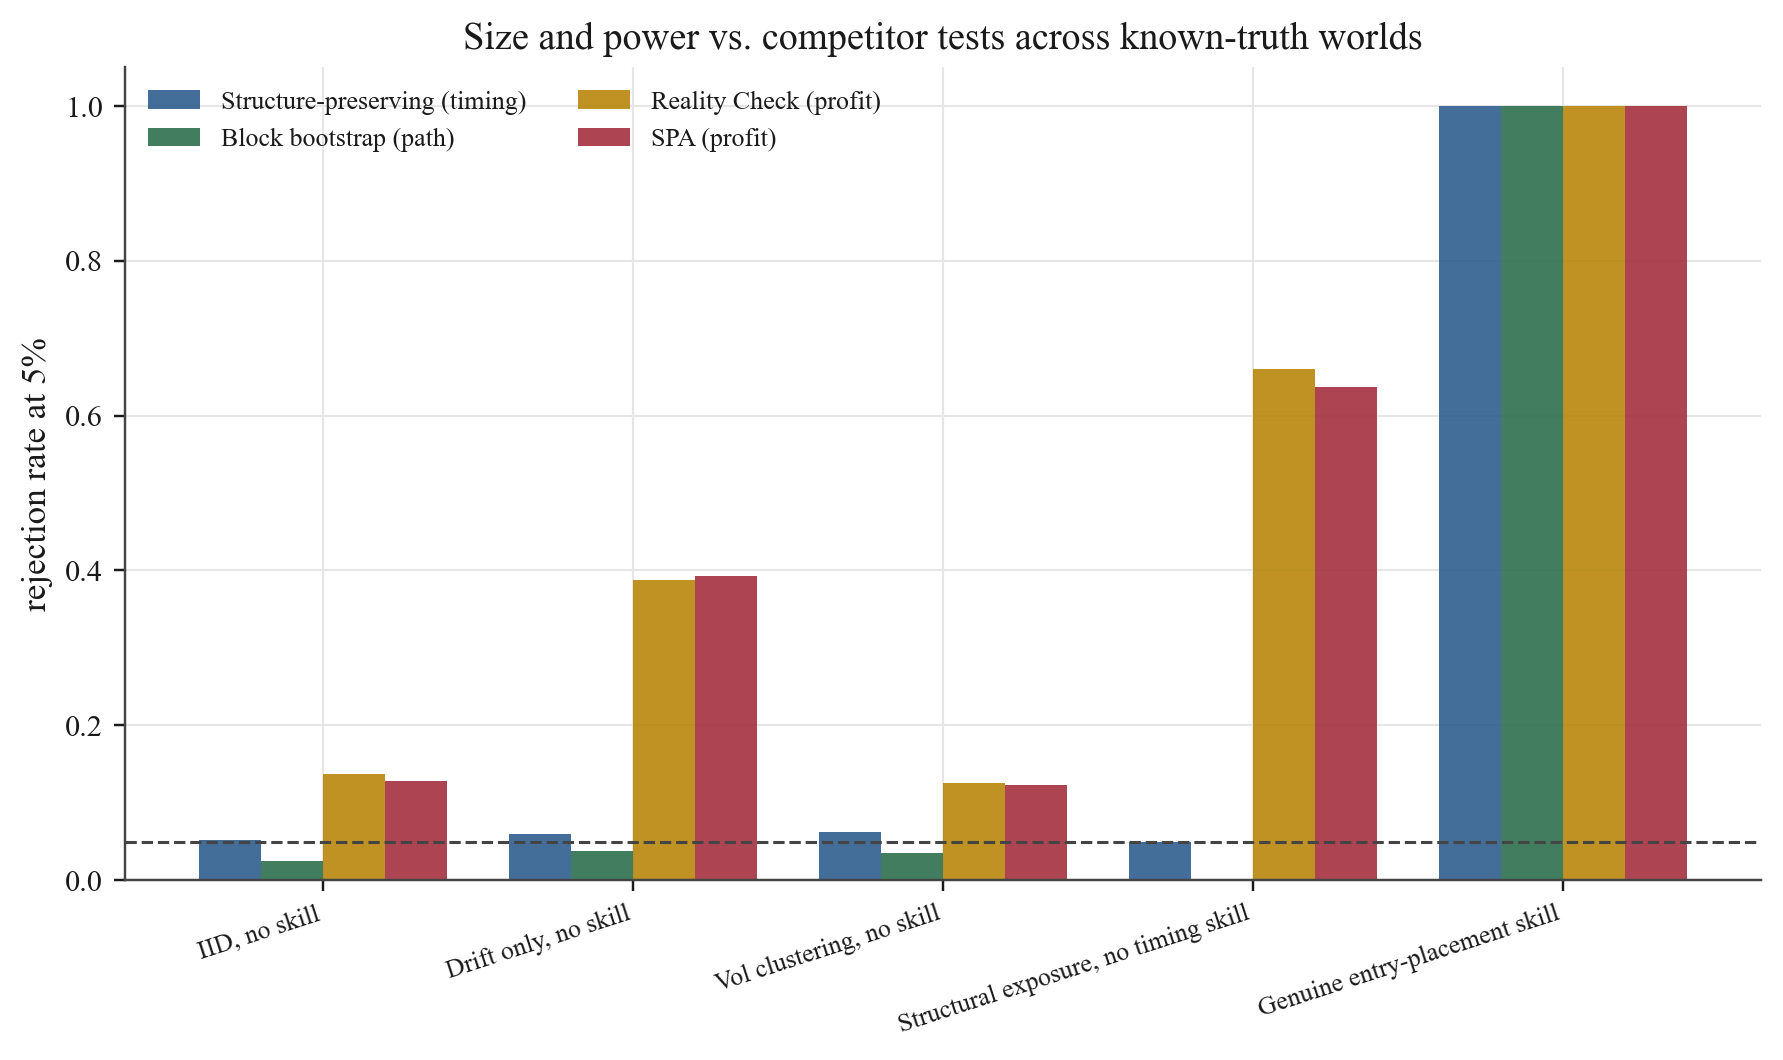
\includegraphics[width=0.92\textwidth]{competitor_comparison.png}
\caption{Rejection rates of the four tests across the five known-truth worlds (dashed line: nominal $5\%$). All four detect genuine entry skill (right). In the no-skill worlds only the structure-preserving and block-bootstrap timing tests hold size; Reality Check and SPA reject a profitable-but-untimed strategy roughly two-thirds of the time (fourth cluster), because they test profitability rather than placement.}
\label{fig:competitor}
\end{figure}

\section{Empirical results}

\subsection{The central panel}

Table~\ref{tab:main} reports the eleven-strategy GC=F panel on the common window 2002-03-04 to 2026-04-02. The pattern is a systematic divergence between profitability and timing evidence. Ten of the eleven strategies post positive cumulative return (realized returns span $-0.010$ to $0.803$) against a buy-and-hold benchmark of $14.670$ that measures how much long-horizon appreciation the sample contained. Yet under the structure-preserving null no strategy crosses $p\le0.05$, before or after Benjamini--Hochberg adjustment; Squeeze Breakout comes closest at $p=0.053$, though with only $N=4$ trades it is exploratory rather than inferential: the asymptotics of Section~\ref{sec:theory} do not apply at $N=4$ and only $3!$ internal-gap arrangements carry placement information, so the placement margin is weakly identified, and exact enumeration of its orbit confirms the non-rejection (Online Supplement, Section~S3). The classifier assigns no moderate or strong skill: four are classified \emph{above median} (not significant), five as \emph{random or luck}, and two as \emph{below null median}. This verdict is under the neutral gap-permutation measure; its dependence on the conditioning choice is the subject of Section~\ref{sec:schedule-sensitivity}.

\begin{table}[t]
\centering
\caption{GC=F daily panel: strategy outcomes and skill diagnostics for the eleven-rule panel over the common window.}
\label{tab:main}
{\small
\renewcommand{\arraystretch}{1.15}
\setlength{\tabcolsep}{5pt}
\begin{adjustbox}{max width=\textwidth}
\begin{tabular}{@{}lrrrrrrl@{}}
\toprule
Strategy & Cum.\ return & Trades & RCSI (mean$\pm$SD) & $p$-value & Percentile & $\mathrm{RCSI}_z$ & Verdict \\
\midrule
Trend Pullback      & 0.083 &  77 & $-0.361\pm0.005$ & 0.870 & 13.0 & -1.03 & Below null median \\
Breakout Vol+Mom    & 0.297 &  46 & $\phantom{-}0.158\pm0.003$ & 0.176 & 82.4 & \phantom{-}0.91 & Above median (n.s.) \\
Mean Rev Vol Filter & -0.010 & 13 & $-0.029\pm0.001$ & 0.662 & 33.8 & -0.44 & Random or luck \\
Validation AVM      & 0.219 &  35 & $\phantom{-}0.059\pm0.003$ & 0.345 & 65.5 & \phantom{-}0.32 & Random or luck \\
ADX Trend           & 0.803 & 110 & $\phantom{-}0.387\pm0.005$ & 0.141 & 85.9 & \phantom{-}1.08 & Above median (n.s.) \\
Oversold Reversion  & 0.082 &  30 & $\phantom{-}0.034\pm0.001$ & 0.341 & 65.9 & \phantom{-}0.35 & Random or luck \\
Squeeze Breakout    & 0.065 &   4 & $\phantom{-}0.055\pm0.000$ & 0.053 & 94.7 & \phantom{-}1.50 & Above median (n.s.) \\
Connors RSI2        & 0.118 &  41 & $\phantom{-}0.094\pm0.001$ & 0.143 & 85.7 & \phantom{-}1.07 & Above median (n.s.) \\
Donchian Reentry    & 0.071 &  60 & $-0.088\pm0.003$ & 0.647 & 35.3 & -0.46 & Random or luck \\
Turn-of-Month       & 0.323 & 141 & $\phantom{-}0.144\pm0.003$ & 0.234 & 76.7 & \phantom{-}0.65 & Random or luck \\
Random              & 0.601 & 215 & $-0.103\pm0.523$ & 0.710 & 29.0 & -0.64 & Below null median \\
\midrule
Buy \& Hold (benchmark) & 14.670 & --- & --- & --- & --- & --- & Benchmark \\
\bottomrule
\end{tabular}
\end{adjustbox}
}
\par\vspace{0.75em}
\begin{minipage}{0.95\textwidth}
\centering
\footnotesize\emph{Notes.} Cum.\ returns are the final cumulative returns for the common window 2002-03-04 to 2026-04-02 (equity curves in Online Supplement~S6). Trades are the counts reported in the strategy-specific Monte Carlo distribution captions. RCSI is reported as mean $\pm$ SD across outer-run seeds (outer runs = 100, simulations per run = 5{,}000, transaction cost = 0.000470; Online Supplement~S5). The verdict and the ($p$-value, percentile, $\mathrm{RCSI}_z$) triple are the classifier-aligned values. The Random baseline's percentile is a single seed-$42$ realization; across $R=100$ outer seeds it averages $48.3\pm25.6$ (Online Supplement~S5), so its single-run rank should not be read as stable.
\end{minipage}
\end{table}

The divergence has a direct cause: gold appreciated over the sample, so any sufficiently long-biased rule captures part of that trend regardless of when it enters, and the structure-preserving null absorbs the drift by repricing the same trades on the same appreciating path. The embedded random baseline makes the point sharpest. The Random strategy enters with probability $0.07$ per bar, ignores every market feature, and is nonetheless profitable at $0.601$, more than nine of the ten rule-based strategies, yet it classifies as \emph{below null median} ($p=0.710$, percentile $29.0$). Its return comes entirely from long exposure to an appreciating asset; its random timing sits near the center of its own null, and the seed-$42$ realization falls just below. Profit without timing information is exactly what the null is built to expose. Per-strategy Monte Carlo summaries, the comparison to return-based alternative nulls, the anatomy of the four above-median strategies, and the seed-robustness of these classifications are reported in the supplement (Online Supplement, Sections~S3 and~S5).

\subsection{Cross-asset breadth under multiplicity control}
\label{sec:cross-asset-multiplicity}

The GC=F panel is one asset. Pooling every completed full-sample test on disk ($322$ strategy-by-asset tests across $47$ instruments) and correcting jointly, no discovery survives Benjamini--Hochberg or Bonferroni control, the raw nominal-rejection count ($13$) is below the $16.1$ expected by chance, and the panel $p$-values skew conservative (mean $0.567$). The clearest sign that the nominal hits are luck is their identity: the smallest $p$-value in the panel ($0.0014$) belongs to a \emph{random}-entry baseline, and random baselines occupy three of the thirteen. This is an availability sample, not a designed universe, and the seed-robust evidence remains single-asset; the panel construction, the exploratory multi-asset walk-forward, and the bounded daily/4-hour/hourly frequency check, all pointing the same way, are in the Online Supplement (Section~S3).

\subsection{Schedule-measure sensitivity}
\label{sec:schedule-sensitivity}

The choice of schedule measure $\mathbb{Q}$ is part of the null hypothesis, so the verdict must be checked against nearby measures. Re-evaluating the full panel under a leading-gap feasibility restriction, forbidding the first simulated entry inside the universal $200$-bar signal warm-up, changes no verdict and crosses no threshold: the headline is robust to the concern that the null might place trades in pre-signal bars a real strategy could not have used. Because the unrestricted measure can otherwise place trades among the cheap early-sample prices of a trending path, it, if anything, inflates the null mean and biases toward non-rejection; the restriction removes that bias and still moves no verdict across the threshold. The picture changes under the context-matched measure, which restricts each random entry to bars whose trailing-volatility context matches the realized entries. On a strongly trending asset this narrow matched pool can earn far more, or far less, than the realized schedule, and four strategies reject at the $5\%$ level (Connors RSI2 at $p<0.001$, ADX Trend at $p=0.010$, Breakout Vol+Mom at $p=0.022$, Squeeze Breakout at $p=0.030$) while four others fall to the floor of the null ($p\approx1$). We do not read these rejections as competing evidence of skill: the neutral gap-permutation measure rejects none of the eleven, so the conjunctive standard, significance under every defensible measure, is settled by that column alone, and a narrow matched pool can in principle sharpen tails in either direction. A second volatility-state measure points the same way. The regime-preserving measure restricts each random entry to bars in the realized entry's forward-safe volatility-regime tercile (calm, neutral, or stressed), a coarser, look-ahead-free discretization of the same trailing-volatility state the context-matched measure bins into quintiles; it rejects the same four strategies (Breakout Vol+Mom at $p=0.037$, ADX Trend at $p=0.012$, Squeeze Breakout at $p=0.032$, Connors RSI2 at $p<0.001$) and no others; the replication rests substantively on the three large-$N$ rules, since Squeeze Breakout at $N=4$ is read as exploratory. Because both measures condition on trailing realized volatility, their agreement does not isolate placement from the volatility-state channel; what it rules out is a binning- or construction-specific matched-pool artifact, and it points to a volatility-regime-conditional placement effect that the neutral measure conditions away. The point is the disagreement itself. A timing verdict that flips between the neutral and the state-preserving schedule measures establishes the absence of \emph{robust, measure-invariant} entry-placement skill, which is the paper's central epistemic claim; we treat agreement across schedule measures, not rejection under any single one, as the right bar for a timing claim, and develop the implications in the discussion. Table~\ref{tab:schedule_sensitivity} reports the full panel under all four measures.

\begin{table}[H]
\centering
\caption{Schedule-measure sensitivity. One-sided Monte Carlo $p$-values for the GC=F panel under the primary gap-permutation measure, a leading-gap restriction (first entry beyond the $200$-bar warm-up), and the context-matched measure, and a regime-preserving measure (each random entry restricted to bars sharing the realized entry's market-regime label). Daggers mark $p\le 0.05$.}
\label{tab:schedule_sensitivity}
{\small
\renewcommand{\arraystretch}{1.12}
\setlength{\tabcolsep}{7pt}
\begin{adjustbox}{max width=\textwidth}
\begin{tabular}{@{}lrrrr@{}}
\toprule
Strategy & Gap-permutation $p$ & Leading-gap $\ge 200$ $p$ & Context-matched $p$ & Regime-preserving $p$ \\
\midrule
Trend Pullback      & 0.870 & 0.910 & 1.000 & 1.000 \\
Breakout Vol+Mom    & 0.176 & 0.128 & 0.022$^\dagger$ & 0.037$^\dagger$ \\
Mean Rev Vol Filter & 0.662 & 0.668 & 0.395 & 0.186 \\
Validation AVM      & 0.345 & 0.303 & 0.993 & 0.986 \\
ADX Trend           & 0.141 & 0.055 & 0.010$^\dagger$ & 0.012$^\dagger$ \\
Oversold Reversion  & 0.341 & 0.383 & 0.146 & 0.117 \\
Squeeze Breakout    & 0.053 & 0.100 & 0.030$^\dagger$ & 0.032$^\dagger$ \\
Connors RSI2        & 0.143 & 0.155 & ${<}0.001^\dagger$ & ${<}0.001^\dagger$ \\
Donchian Reentry    & 0.647 & 0.671 & 1.000 & 1.000 \\
Turn-of-Month       & 0.234 & 0.320 & 1.000 & 1.000 \\
Random              & 0.710 & 0.713 & 1.000 & 1.000 \\
\midrule
Significant at $5\%$ & 0 of 11 & 0 of 11 & 4 of 11 & 4 of 11 \\
\bottomrule
\end{tabular}
\end{adjustbox}
}
\end{table}


\section{Discussion}
\label{sec:discussion}


\subsection{The measure family as the inferential object}
\label{sec:discussion-measure}

The most serious objection to the procedure is not that any particular verdict is
wrong but that the verdict is defined relative to a choice the analyst makes, and we
take that dependence as the central point. The null is indexed by a conditioning
measure $\mathbb{Q}_\theta$ drawn from the family
$\mathfrak{Q}=\{\mathbb{Q}_\theta:\theta\in\Theta\}$ of Section~\ref{sec:theory}; all
members fix the realized path $\{P_t\}$ and the structural profile $\mathcal{S}$, and
they differ only in which additional features $M_\theta$ of the realized schedule
they hold fixed. That choice is not pinned down by the data. It is a modeling
decision on the same footing as the specification of a regression or the choice of an
instrument, and it should be declared and defended as one; in the language of risk
analysis it is a source of model risk, and the sensitivity range across $\Theta_0$ is
its quantification. Each $\mathbb{Q}_\theta$ carries its own null $H_0^\theta$ and its
own estimand $q_\theta=\mathbb{Q}_\theta\big(T(S)\ge T(S_0)\big)$, so the reported
quantity is not a single verdict but a \emph{sensitivity range} of measure-specific
verdicts, one per admissible $\theta$. The object of inference is therefore that
range, and the analyst's task is to specify the admissible class $\Theta_0$ over
which it is to be read, that is, to declare, in advance, which partitions of the
realized record into ``structure'' and ``placement'' are defensible for the question
at hand. These are outer bounds over a finite, analyst-chosen menu, not a sharply
identified set in the Manski sense \cite{Manski2003,Tamer2010}.

Stating $\Theta_0$ in advance is what turns a free parameter into a model, and it is
what gives the sensitivity-range language of Section~\ref{sec:theory} its content.
The width of the range across $\Theta_0$ is the relevant robustness statement: a
verdict that is constant across the admissible class is robust to the partition, and
one that flips is reported only as a range whose elements disagree. We define
\emph{measure-invariant entry-placement skill} as rejection of $H_0^\theta$ for every
$\theta\in\Theta_0$, and we adopt agreement across $\Theta_0$ as the bar a timing
claim must clear. The reason is not conservatism for its own sake but identification.
Because the measures differ precisely in where they draw the structure/placement
line, a rejection under $\mathbb{Q}_\theta$ but not $\mathbb{Q}_{\theta'}$ is
confounded with the conditioning choice $\theta$; only invariance to that choice
isolates placement as opposed to the analyst's partition. Measure invariance is thus
a strictly stronger and more credible claim than rejection under any single
hand-picked measure, and it is the right standard for a timing claim because the
timing question is exactly the question that the structure/placement partition is
meant to answer.

Two boundaries of this standard must be stated plainly, and only once. Invariance is
\emph{necessary but not sufficient}: a confound shared by every admissible measure
would survive across $\Theta_0$, so agreement bounds the set of explanations but does
not collapse it to skill. And invariance is \emph{not necessary} for informative
placement, because a conditioning measure can absorb real state-conditional skill into
the structure it holds fixed; a strategy that times entries well only within a market
state which the measure matches on will, correctly under that measure's null, fail to
reject. The schedule-measure sensitivity of Section~\ref{sec:schedule-sensitivity}
illustrates this dependence directly. The neutral gap-permutation measure rejects none
of the eleven strategies, while two volatility-state measures reject the same four: the context-matched measure, restricting random
entries to bars in the same trailing-volatility quintile, and the regime-preserving measure, restricting them to bars in the same forward-safe volatility-regime tercile, both reject Connors RSI2,
ADX Trend, Breakout Vol+Mom, and Squeeze Breakout and no others (Table~\ref{tab:schedule_sensitivity}). The disagreement locates the
verdict's dependence on $\theta$ at a specific, interpretable margin: whatever
advantage those four strategies show is inseparable, on this evidence, from a
volatility-state alignment that the context-matched measure either credits as
placement or conditions away as structure, depending on which side of the line one
draws. Because no strategy rejects under the neutral measures while the same four reject under both state-preserving measures, the sensitivity range of
verdicts contains both ``skill'' and ``no skill'' for those four, and the conjunctive
standard returns the honest reading: the absence of robust, measure-invariant
entry-placement skill, with the disagreement marking where state-conditional
placement information lives. The replication is informative, with a stated limit. Both measures condition on trailing realized volatility, so their agreement does not isolate placement from the volatility-state channel; what it rules out is a binning- or construction-specific matched-pool artifact, since a coarse forward-safe regime tercile and a finer in-sample volatility quintile agree on exactly the same four. The data therefore partially adjudicate the margin: for these four volatility-filtered strategies the edge is volatility-state-conditional and robust to how that state is discretized, which is the non-necessity of Proposition~\ref{prop:nonsuff}(ii) made empirical. What the data do not deliver is measure-invariant skill, since no edge survives the neutral, regime-agnostic measure; the headline claim, no robust, measure-invariant entry-placement skill, therefore stands, and Remark~\ref{rem:necessity} records that it is a falsification, not a certification. Measure-dependence is the form in which the procedure reports what the
data can and cannot identify.

This worst-case-over-a-set posture is the one familiar from robust risk
measurement. Coherent and convex risk measures evaluate a position as a supremum of
expected loss over a set of probability measures \cite{ArtznerDelbaenEberHeath1999}
(the resemblance is to that worst-case-over-a-set form, not to the coherence axioms:
our $\Theta_0$ is a finite menu and we take no convex mixture of measures, so the
construction is not itself a coherent risk measure); robust decision theory scores a
policy at its least-favorable model \cite{HansenSargent2008}; and model uncertainty
about the pricing measure is the object formalized for derivatives by
\cite{Cont2006}. The decision-theoretic primitive behind this worst-case posture is maxmin expected utility over a set of priors \cite{GilboaSchmeidler1989}, though our use is inferential rather than decision-theoretic: the supremum is taken over the admissible conditioning measures of a test, and the declared menu $\Theta_0$ plays the role of the prior set, not of subjective beliefs. The intersection--union test of Section~\ref{sec:theory} is the
inferential analogue at the level of form: the measure-invariant verdict is the one
that survives the least-favorable admissible conditioning measure, and the
sensitivity range $[\min_\theta q_\theta,\max_\theta q_\theta]$ is the model-risk
interval the choice of null induces. Reporting an interval of admissible probabilities in place of a single number is the posture of imprecise probability \cite{Walley1991}, though our menu is a finite, analyst-enumerated set of designs, deliberately not a convex credal set. The least-favorable structure of
Proposition~\ref{prop:minimax} supports the analogy at the level of form, not as an
exact optimality identity: the power of the intersection--union rule is bounded by
its least-favorable admissible measure, just as a robust criterion is bounded by its
least-favorable model. We do not claim the rule attains that bound or solves a
maximin game; the test is built to detect the intersection alternative
(measure-invariant skill), and reading $\Theta_0$ as a declared worst-case menu
rather than a single hypothesized truth is what places the construction alongside
worst-case-over-a-set decision rules rather than alongside point identification. We do not overstate the construction's current reach: the
admissible menu we operate, $\Theta_0=\{$gap-permutation, leading-gap,
context-matched$\}$, is a small, explicitly enumerated set on a single asset, so the
reported range illustrates the machinery rather than delivering a rich identified set;
enlarging $\Theta_0$, and sampling the uniform-feasible and slack-redistribution
measures of Table~\ref{tab:schedule_measures} once their structural profile is
coarsened to admit them, is the natural next step.

\subsection{Limitations and failure modes}
\label{sec:limitations}

We have stated the central caveat already: the verdict is defined relative to a
conditioning measure the analyst chooses, and what the data return is a sensitivity
range, not a scalar (Section~\ref{sec:discussion-measure}). That caveat is the
governing one, but it is not the only place the procedure can be pressed. We
therefore set out, plainly and without hedging, the failure modes a careful reader
should hold the method to. Some have a repair, which we give; others are scope
limitations we accept rather than fix; a few would require computations we have not
run, which we flag as such and do not report. None of them moves a reported number,
and we are explicit about which weaknesses the body of the paper already addresses.

\paragraph{Exactness is exactness against a sharp null, not a property of the
procedure.} The finite-sample validity of Theorem~\ref{prop:q-validity}(i)
holds under the hypothesis that the realized statistic $T(S_0)$ is exchangeable with
its $\mathbb{Q}_\theta$-resamples given $\mathcal{C}$. This is the content of the
null $H_0$ of Definition~\ref{def:h0} and its measure-indexed form $H_0^\theta$, not a guarantee the procedure confers
on arbitrary data: $\mathbb{Q}_\theta$ is an analyst-chosen reference law, and under
any alternative the realized schedule was generated by a rule, so it is not a
$\mathbb{Q}_\theta$-draw. The contrast with the model-X construction of
\cite{Candes2018} is instructive and unflattering: there the conditional law of the
covariate is known by design, so exchangeability is guaranteed; here it is named and
conditioned on. The procedure therefore tests the discrepancy between the realized
placement and the chosen reference law; it does not certify that the reference law is
the correct counterfactual. We have stated this in
Section~\ref{sec:fs-validity}, and we use the phrase ``exact against $H_0^\theta$''
rather than ``exact'' without qualifier throughout. The limitation we accept is that
the word ``exact'' carries an unconditional connotation it does not earn here, and a
reader should append the qualifier wherever the abstract or introduction omits it for
brevity.

\paragraph{The asymptotic theory rests on a condition we impose rather than verify.}
The consistency, minimum-detectable-edge, and local-power results
(Theorem~\ref{prop:consistency}, Corollary~\ref{prop:local-power}) are
conditional on Assumption~\ref{ass:clt}, a central-limit condition for a statistic
that is a gap-permutation of one fixed, autocorrelated, heavy-tailed path. This is a
genuinely hard object: the per-trade contributions are functions of the permutation,
not a fixed array, so Hoeffding's combinatorial central-limit theorem is a motivating
analogy rather than a sufficient theorem, as Section~\ref{sec:theory} already states.
We do not claim to have verified Assumption~\ref{ass:clt} for the gold path. The
conditions (a) no-dominant-term and (b) weak dependence are sufficient and imposed,
and they can fail: when one or a few trades dominate the return budget, (a) is
violated, the Gaussian approximation degrades, and the standardized statistic is not
pivotal. Two consequences follow. First, $\mathrm{RCSI}_z$ is descriptive and only
approximately pivotal under Assumption~\ref{ass:clt}, never the carrier of the
verdict; the verdict rests on Theorem~\ref{prop:q-validity}(i), which needs no
central-limit condition. Second, the Kolmogorov--Smirnov uniformity tests of
Section~\ref{sec:simulation-validation} probe calibration of the $p$-value, which
follows from exchangeability, and not the normality of $Z_N$, which they cannot
confirm; we read them only as evidence on calibration. A combinatorial central-limit
theorem matched to the actual statistic, for permutation sums whose summands depend on
the permutation under mixing, would replace the assumption with a result; locating
such a theorem in the mixing permutation-CLT literature, and verifying it applies, is
left for future work, and we do not assert a citation we have not confirmed exists.

\paragraph{At small trade counts the conditioning measure isolates little placement
information.} For low-$N$ strategies the gap-permutation orbit is dominated by the
leading-gap draw. On a trending path the leading gap is close to a monotone function
of calendar position, hence an exposure channel rather than a placement channel, while
the internal-gap permutation, the component that tests spacing, is degenerate at $N=2$
and weak for small $N$. For such strategies the estimand reflects where the template's
first entry sat in calendar time more than how its trades were spaced. We therefore
read small-$N$ verdicts as exploratory not only because the asymptotics of
Assumption~\ref{ass:clt} are out of force (Section~\ref{sec:mde}) but because the
conditioning measure isolates little placement information to begin with. The
leading-gap restriction of Section~\ref{sec:schedule-sensitivity} removes the
cheap-early-price channel but cannot restore spacing information the small orbit does
not contain. This upgrades the existing ``exploratory at small $N$'' reading from a
statement about power to a statement about identification: at $N=4$ (Squeeze Breakout,
Table~\ref{tab:main}) and comparable counts, non-rejection is uninformative on both
grounds. Small-$N$ strategies in fact face three compounding penalties that the paper
should keep distinct: the tied-gap orbit makes the test strictly conservative
(Theorem~\ref{prop:q-validity}(i)), the small trade count inflates the minimum
detectable edge (Theorem~\ref{prop:consistency}), and the leading-gap draw
dominates the estimand. We draw no inference from their non-rejection.

\paragraph{The conditioning set can absorb skill, and ``lower bound'' is the wrong
word for what survives.} The holding-duration multiset $\mathbf{h}$ and the
internal-gap multiset $\mathbf{g}^{\mathrm{int}}$ are themselves outputs of the
strategy's decision rule, so conditioning on them attributes any edge that lives in
exit logic or holding-period selection to the structure rather than to placement
(Section~\ref{sec:conditioning-estimand}). Two refinements of that already-stated
caveat are warranted. First, because Algorithm~\ref{alg:spr} reattaches a permuted gap
sequence to the durations in their realized order, the test isolates a placement
margin net of any entry-duration interaction: an edge residing in the joint choice of
when to enter and how long to hold is charged to the conditioned structure, not to
placement, and can be neither manufactured nor recovered by the placement contrast.
Second, the term ``lower bound on total strategy skill'' overstates what holds. A
lower bound is a number that no realized skill can fall below; nothing here is bounded,
because $\mathbf{h}$ and $\mathbf{g}^{\mathrm{int}}$ can absorb an arbitrary share of
the edge with no floor. The correct statement, and the one
Proposition~\ref{prop:nonsuff}(ii) already supports, is that non-rejection is
consistent with skill residing in the conditioned dimensions or in their interaction
with placement; it is not a numerical lower bound but a statement that, within the
placement margin the chosen measure exposes, no edge is detected. We accordingly avoid
the phrase ``lower bound'' and read non-rejection as silence about the conditioned
dimensions, not as a floor on skill.

\paragraph{Holding durations are kept in realized order while gaps are permuted; the
asymmetry is a modeling choice.} Algorithm~\ref{alg:spr} preserves which trade is long
and which is short, in sequence, but scrambles spacing. The asymmetry is deliberate:
the strategy's exit logic, encoded in the ordered durations, is treated as part of the
fixed structure, while spacing is the discretionary placement margin under test. We
state this here because the choice is not self-justifying, and a reader could equally
defend a measure that permutes the durations, or one that permutes the duration-gap
pairs jointly to preserve their realized pairing. Each such measure is a further member
of the family of Definition~\ref{def:measure-family} and, by the menu-monotonicity
already noted there, would only widen the reported sensitivity range. Evaluating a
duration-permutation measure and a joint duration-gap-pairing measure on the panel
remains to be run against the implementation; we therefore do not report verdicts under
them, and we note only that their omission makes the reported range narrower than the
fullest defensible menu would give.

\paragraph{Atomicity at small $N$ arises only when internal gaps tie, and Squeeze Breakout is not such a case.} When internal gaps contain ties, including the zero-gap same-bar transitions
Algorithm~\ref{alg:spr} preserves, the number of distinct feasible schedules falls
below the nominal count of internal-gap permutations times leading-gap values, and the
support of $T$ can collapse onto few atoms; the effective $p$-resolution is then set by
the distinct-schedule count rather than by the Monte Carlo budget. The $N=4$ Squeeze
Breakout strategy is \emph{not} such a case. Its internal gaps are distinct, so exact
enumeration gives $6\times471=2{,}826$ feasible schedules with $2{,}826$ distinct
statistic values and an exact one-sided tail probability of $0.057$ under the
deterministic-cost gap-permutation null (Online Supplement, Section~S3), consistent with
the Monte Carlo $p=0.053$ and likewise short of significance. Its near-threshold reading
therefore rests on weak identification at $N=4$, not on a coarse grid. Where the orbit is small enough, exact enumeration replaces the Monte Carlo estimate
with the exact tail area, as done above for $N=4$; where enumeration is infeasible we
read the Monte Carlo $p$-value as a tail-area estimate.

\paragraph{Near-flat path windows can make the null dispersion degenerate.} The
statistic is the cumulative return of the template repriced on the path, so if a
randomized trade lands on a locally flat stretch its contribution is near zero by
construction. For short-duration templates on a path with flat patches, many draws can
return nearly identical statistics, the null dispersion can approach zero, and the
percentile then becomes sensitive to negligible return differences. The
$\mathrm{RCSI}_z$ effect size already handles exact zero dispersion by definition
(it is set to zero when the realized return equals the null mean and is otherwise
undefined, Section~\ref{sec:conditioning-estimand}), but the $p$-value under near-zero
dispersion is not separately discussed. The liquid daily GC=F path is unlikely to
trigger this, but the broader cross-asset panel of
Section~\ref{sec:cross-asset-multiplicity} spans instruments where thin or flat windows
are possible. We flag any strategy whose null dispersion is near zero as
path-degenerate and do not interpret its percentile; a dispersion scan across the full
panel to identify such cases remains to be run against the implementation, so we report
no count of affected tests.

\paragraph{The neutral measure may be misspecified for regime-filtered strategies, and
this bears directly on the four context-matched rejections.} Several panel strategies
embed an explicit volatility or regime filter, so their realized gap structure is
correlated with market state. The gap-permutation measure permutes gaps without regard
to state, hence it can place a trade into a volatility window the strategy would never
have entered. A reader can argue that, for such strategies, the regime occupancy is
itself part of the structure, the context-matched measure is the correct null, and the
four context-matched rejections (Connors RSI2 at $p<0.001$, ADX Trend at $p=0.010$,
Breakout Vol+Mom at $p=0.022$, Squeeze Breakout at $p=0.030$,
Table~\ref{tab:schedule_sensitivity}) are genuine state-conditional placement skill
rather than matched-pool artifact. The data partially adjudicate this, as the regime-preserving measure below shows: it is
exactly the non-necessity of Proposition~\ref{prop:nonsuff}(ii), and
Remark~\ref{rem:necessity} already records that the headline is a falsification, not a
certification. The honest statement is therefore narrower than ``no skill'': no edge
survives the neutral, regime-agnostic gap-permutation measure, and the
regime-conditional channel remains open as a skill question, since a state-preserving measure can replicate the rejections but cannot certify skill. The measure that would arbitrate them, the regime-
or block-preserving measure listed in Table~\ref{tab:schedule_measures}, has now been
evaluated (Section~\ref{sec:schedule-sensitivity}): restricting each random entry to
bars sharing the realized entry's regime label, it rejects the same four strategies as
the context-matched measure and no others. Both measures condition on trailing realized volatility, so the four rejections replicate
across two discretizations of the same volatility state, a forward-safe regime tercile and an
in-sample volatility quintile; this makes a binning- or construction-specific matched-pool
artifact unlikely but does not isolate placement from the volatility-state channel. The
rejections remain absent under the neutral measure, so measure-invariant skill still fails.

\paragraph{The measure-invariant standard is low-power by construction, so its
non-rejection is weak evidence.} Corollary~\ref{cor:iut-power} bounds the power of the
intersection--union test by the least-favorable measure, and Section~\ref{sec:theory}
already states that this power can be near zero whenever admissible measures disagree.
The interpretive consequence deserves to be foregrounded rather than buried in the
power analysis: ``no robust, measure-invariant entry-placement skill'' is the
non-rejection of a standard that is near-powerless the moment the admissible menu
contains two measures that ever disagree, which on this panel it does. A non-rejection
of a deliberately low-power standard is not evidence of absence, and the measure-
invariant verdict should be read as a consequence of the conjunctive standard, not as a
finding about gold. The substantive, powered result is the single-measure one: under
the neutral gap-permutation measure, which the real-path positive control of
Section~\ref{sec:simulation-validation} shows is powered to detect injected timing skill
on the gold path (the baseline sits at the $50.5$th percentile and power rises
monotonically with injected skill), no strategy in the panel rejects, and across the
$322$-test cross-asset panel nothing survives multiplicity control
(Section~\ref{sec:cross-asset-multiplicity}). We foreground that powered single-measure
non-rejection and demote the measure-invariant verdict to a consequence of the standard;
Remark~\ref{rem:necessity} licenses exactly this reading.

\paragraph{The competitor comparison demonstrates a difference in questions, not a
defect in the competitors.} Table~\ref{tab:competitor} shows the structure-preserving
test holding size at $0.050$ in the structural-exposure world while the single-strategy
specializations of Reality Check and SPA reject at $0.660$ and $0.638$. As
Section~\ref{sec:competitor} already states, this is not an error by those procedures:
a test of profitability should reject a profitable strategy, and the demonstration is
that profitability and placement are different objects, which
Theorem~\ref{prop:orthogonality} formalizes. We retain that framing and do not
present the competitors' rejections as failures of their own design. One small honesty
point about our own size: in the same controlled worlds the structure-preserving test
ranges from $0.050$ to $0.063$ across no-skill worlds, and the $0.063$ figure under
volatility clustering sits modestly above nominal relative to the reported Monte Carlo
standard error of $0.011$ (Section~\ref{sec:competitor}). Volatility clustering is
precisely the regime that stresses the mixing condition (b) of
Assumption~\ref{ass:clt}. We therefore claim approximate calibration under clustering,
not exact size, and we do not assert that the test holds nominal size under arbitrarily
strong dependence.

\paragraph{Smaller specification points.} A few narrower issues we record rather than
resolve. The transaction-cost cancellation of Section~\ref{sec:conditioning-estimand}
is approximate, not pathwise exact: a percentage cost levied on randomized placements
couples to the price level, so on a trending path the cancellation holds in expectation
but the realized cost differs across placements; the direction of the residual still
favors non-rejection, as stated there. The $\mathrm{RCSI}_z$ classifier input is
undefined when the null dispersion is exactly zero and the realized return differs from
the null mean; this is the path-degenerate edge case above, and we treat such a
strategy as flagged rather than classified. The $322$-test panel
(Section~\ref{sec:cross-asset-multiplicity}) is an availability sample, so its multiplicity
control governs the tests run, not the selection of which assets completed; the paper
already labels it an availability sample and reports that the smallest panel $p$-value
($0.0014$) belongs to a random-entry baseline, which is itself the cleanest sign that
the nominal hits are chance, but the selection mechanism is not modeled and we do not
treat the panel as exchangeable across assets. Finally, the trend mechanism behind the
``below null median'' labels (Trend Pullback, Random in Table~\ref{tab:main}) is
benign but worth naming: on an appreciating path the null mean averages the template
over calendar positions, so a strategy's rank partly reflects where in calendar time
its template sits relative to a uniform spread, and a ``below null median'' label
should be read as ``entered earlier than a uniform calendar spread on an appreciating
asset,'' not as negative timing skill. For large-$N$ strategies the internal-gap
permutation dominates the randomness and this calendar-position channel is small; for
small-$N$ strategies it is not, which is a further reason their verdicts are
exploratory.

\subsection{Economic significance}
\label{sec:discussion-economic}

The finding has an economic reading. Across the panel, entry-timing performance
is largely not separately identifiable from structural exposure to a drifting asset: to
first order the realized return is reproducible by randomized placement of the same trades.
For performance attribution and manager due diligence, a profitable track record is on its
own uninformative about timing skill, so an allocator should require a timing claim to
clear a structure-matched counterfactual before paying for it; the test supplies that
instrument, requiring no return model and computable from a trade log. For the
market-efficiency reading, the result sharpens the object of study: rather than asking
whether a strategy beats a benchmark, it isolates the placement margin most often mistaken
for skill and finds it scarce and measure-fragile even where profitability is common. For
strategy development, the diagnostic screens out rules whose apparent edge is conditioned
away as structural exposure and so will not survive live trading on a different path. We
restrict the claim accordingly: because the test refutes rather than certifies
(Section~\ref{sec:theory}), it is a screening diagnostic, not an allocation signal, and a
non-rejection is evidence of absence only where the design is powered (Section~S2).

\subsection{Beyond entry timing}
\label{sec:discussion-general}

The construction is not tied to entry timing, long-only trading, or gold. It
applies whenever a decision sequence is overlaid on an exogenous process and one wishes to
separate the marginal contribution of the decisions from the structural exposure they
create: hold the structural footprint fixed, randomize only the decision margin, and refer
the realized statistic to the law this induces. Replacing ``entry placement on a price
path'' with the analogous decision--structure pair yields a test for factor-timing and
tactical asset-allocation rules (randomize the rebalancing schedule while holding portfolio
weights and the realized factor path fixed), for execution algorithms in the small-impact
regime (randomize child-order placement while holding the parent order and the realized
microstructure path fixed, a transfer that requires the orders themselves not to move the
path, and so is restricted to that regime), for the evaluation of reinforcement-learning and
agentic policies (randomize action timing while holding the policy's structural footprint
fixed, scoring against a structure-matched random policy), and for the timing of macro
forecasts and event signals (randomize the announcement-relative placement). In each case
the same three ingredients recur (a fixed exogenous path, a preserved structural profile,
and a randomized decision margin), so the finite-sample validity of
Theorem~\ref{prop:q-validity}, the local-power and orthogonality results of
Section~\ref{sec:theory}, and the calibration machinery transfer, subject to a domain-specific
feasibility and exchangeability check, and the measure family of
Section~\ref{sec:discussion-measure} returns as the object to specify. We develop the trading-timing instance in full and note these
as directions the same construction supports.


\section{Conclusion}

The relevant object of inference in evaluating a decision sequence is not its
realized payoff but the contribution of the decisions relative to a counterfactual
that carries the same structural burden on the same path. Structure-preserving
randomization inference supplies that counterfactual as a finite-sample valid
conditional test, makes the conditioning measure an explicit, declared modeling assumption, and, because
the measure is a choice, returns a sensitivity range of measure-specific verdicts rather
than a single number, with measure invariance the strongest claim the design supports.

Applied to daily gold futures, profit is common but
robust, measure-invariant entry-placement skill is absent: no strategy clears
$p\le0.05$ under the neutral measure, the verdict reverses under two state-preserving measures (context-matched and regime-preserving), and across an availability sample of $322$ strategy-by-asset tests on $47$ instruments
nothing survives multiplicity control, though the seed-robust evidence is single-asset. Synthetic worlds and a real-path positive control
confirm the test is correctly sized and powered, and the head-to-head comparison
shows where return-based tests, which ask about profitability rather than placement,
credit a profitable-but-untimed strategy. The reading is not that the strategies are
bad but that, within the scope of the timing test, realized profitability is not
separately identifiable from structural exposure.

The construction extends beyond the trading application. Wherever a decision sequence is overlaid on an
exogenous process (factor and allocation timing, execution scheduling, the
evaluation of learned policies, the timing of forecasts), the same recipe holds
the structural footprint fixed, randomizes the decision margin, and refers the
realized statistic to the law this induces. The validity, local-power, and
measure-sensitivity results transfer, subject to a domain-specific feasibility check, and the
measure family returns as the object to specify.


\appendix

\section{Proofs}
\label{app:proofs}

This appendix collects the longer proofs of the propositions in Section~\ref{sec:theory}; the short proofs (finite-sample validity, the intersection--union test, and its power corollary) are given in place.

\begin{proof}[Proof of Theorem~\ref{prop:consistency}]
Under Assumption~\ref{ass:clt}, $Z_N=(T(S_0)-\mu_{\mathbb Q})/\sigma_{\mathbb
Q}\to_d N(0,1)$ when $H_0^\theta$ holds. The location-shift alternative adds a
\emph{deterministic} mean to each contribution: $E[\log(1+CR)]$ moves from
$\mu_{\mathbb Q}$ to $\mu_{\mathbb Q}+N\mu_1$, while the centering and scaling
$(\mu_{\mathbb Q},\sigma_{\mathbb Q})$ are fixed functionals of $\mathbb{Q}_\theta$
and $\mathcal C$. Subtracting the null mean and dividing by $\sigma_{\mathbb Q}$
therefore displaces the standardized statistic by the deterministic amount
$\delta_N=N\mu_1/\sigma_{\mathbb Q}$, leaving an $O_p(1)$ fluctuation governed by
the same limit law; this last step is licensed by the alternative-law clause of
Assumption~\ref{ass:clt}, under which $Z_N-\delta_N\to_d N(0,1)$, so the residual
is genuinely $O_p(1)$ and Gaussian rather than assumed so. Writing
$\delta_N=\sqrt N\,(\mu_1/\sigma_1)\cdot(\sqrt N\,\sigma_1/\sigma_{\mathbb Q})$ and
using $\sigma_{\mathbb Q}\asymp\sqrt N\,\sigma_1$ (the no-dominant-term regime of
Assumption~\ref{ass:clt}(a), under which the variance accumulates linearly in $N$)
gives $\delta_N\asymp\sqrt N\,\zeta\to\infty$. The upper-tail probability
$q_\theta=\Pr_{\mathbb Q}(Z\ge Z_N)$ then tends to zero, and
Theorem~\ref{prop:q-validity}(ii) makes $\hat p_M$ track it. Fixing the
noncentrality $\sqrt N\,\zeta$ at the value delivering a target power inverts to
$\zeta_{\min}\asymp N^{-1/2}$. No circularity arises: validity
(Theorem~\ref{prop:q-validity}) is used only through part~(ii), the deterministic
$M\to\infty$ limit of $\hat p_M$, which holds for any fixed $S_0$ and does not
presuppose the alternative.
\end{proof}

\begin{proof}[Proof of Corollary~\ref{prop:local-power}]
By Theorem~\ref{prop:consistency} the deterministic displacement is
$\delta_N=N\mu_1/\sigma_{\mathbb Q}=\sqrt N\,\zeta_N\cdot(\sqrt N\,\sigma_1/
\sigma_{\mathbb Q})\to h$ along $\zeta_N=h/\sqrt N$, because the second factor
tends to $1$ under the no-dominant-term scaling. Adding a deterministic mean shift
$\delta_N\to h$ to a statistic whose centered form converges to $N(0,1)$ under the
alternative clause of Assumption~\ref{ass:clt} shifts the limit to $N(h,1)$ by
Slutsky's theorem. Therefore
$\Pr(Z_N\ge z_{1-\alpha})\to1-\Phi(z_{1-\alpha}-h)=\Phi(h-z_{1-\alpha})$. The three
values follow by substitution; $\Phi(z_{0.80})=0.80$ gives the stated
$h\approx2.49$.
\end{proof}

\begin{proof}[Proof of Theorem~\ref{prop:orthogonality}]
(i) By definition, under a pure-exposure alternative the conditional placement law
$\mathbb{Q}_\theta(\cdot\mid\mathcal C)$ is unchanged, so the realized schedule
$S_0$ is exchangeable with $S_1,\dots,S_M\sim\mathbb{Q}_\theta$ given $\mathcal C$:
profitability comes from the exposure common to all structurally matched
placements on the path, not from where the trades sit, so the realized statistic
$T(S_0)$ is distributed as a $\mathbb{Q}_\theta$-draw.
Theorem~\ref{prop:q-validity}(i) then gives
$\Pr(\hat p_M\le\alpha\mid\mathcal C)\le\alpha$: the SP rejection probability stays
at the nominal level. This level control is finite-sample and uses only
exchangeability; we do not decompose $T(S_0)$ into an exposure component and a
placement component, and the conclusion needs no such additive split. Under
Assumption~\ref{ass:clt} the asymptotic statement is then immediate: a central draw
has limiting law $N(0,1)$, so the noncentrality of $Z_N$ is zero. The return-mean
statistic $\sqrt N\,\bar d$, by contrast, is centered at the realized mean trade
return, which the exposure raises above the fixed zero benchmark; under
Assumption~\ref{ass:clt} its noncentrality is therefore strictly positive and grows
like $\sqrt N$, so RC/SPA reject with probability tending to one. (ii) Under a
shared per-trade location shift the placement carries a common mean displacement;
provided the per-trade return variance standardizing the two statistics agrees to
leading order under that model, Corollary~\ref{prop:local-power} delivers it into
the $z$-standardized SP statistic and the studentized return-mean statistic as the
same leading noncentrality $h$, so to first order their local powers coincide and
neither dominates. That equal-leading-variance condition is exactly what licenses
the \emph{same} $h$ rather than merely two positive noncentralities. Relative
efficiency beyond this shared leading noncentrality is left for future work:
equality of the full local-power functions would require matching the two variance
functionals against placement, which holds only under the shared-location model.
\end{proof}

\begin{proof}[Proof of Proposition~\ref{prop:nonsuff}]
(i) Suppose a feature $C$ correlated with high realized return is held fixed
(hence not randomized) by every $\mathbb{Q}_\theta\in\mathfrak Q$. Then $C$
contributes identically to $T(S_0)$ and to each $T(S)$ under every measure; if $C$
also displaces $T(S_0)$ upward relative to the resampled placements, because the
realized schedule's interaction with the common conditioned feature is
favorable, then $q_\theta$ is small for all $\theta$, so $H_0^\theta$ is rejected
for all $\theta$, yet the displacement is attributable to $C$, a confound shared
by the whole class, not to placement. The intersection cannot separate a
placement effect from a common-to-all-measures confound. (ii) Take a strategy
whose edge is genuinely conditional on a market state $V$ (e.g.\
trailing-volatility regime). The context-matched measure $\mathbb{Q}_{\theta'}$
restricts resampled entries to bars matching the realized $V$-context; under
$\mathbb{Q}_{\theta'}$ the realized schedule competes only against placements
sharing its state, so the state-conditional edge is held fixed rather than tested,
and $T(S_0)$ is a central draw: $q_{\theta'}$ is not small and $H_0^{\theta'}$ is
not rejected, even though the strategy's placement is genuinely informative
conditional on that state. Hence unanimity fails despite real skill.
\end{proof}

\section{Data and implementation}
\label{app:data}

The primary analysis uses daily gold futures (GC=F) over 2002-03-04 to 2026-04-02;
the buy-and-hold cumulative return over the window is $14.670$. All strategies and
their Monte Carlo null paths share an expected round-trip transaction cost of
$c=0.000470$ in return units, calibrated to daily execution and held fixed at higher
frequencies. The panel comprises eleven rules (Trend Pullback, Breakout Vol+Mom,
Mean Rev Vol Filter, Validation AVM, ADX Trend, Oversold Reversion, Squeeze
Breakout, Connors RSI2, Donchian Reentry, Turn-of-Month, and a Random control), with
thresholds fixed before the reported run and applied identically across assets. The
data pipeline, forward-safe regime labeling, next-bar execution and fill model,
strategy rule definitions, the verdict classifier, the Monte Carlo and seed-robustness
protocols, and the full reproduction commands are in the Online Supplement
(Sections~S1 and~S7); code and derived data are archived at
\url{https://github.com/ampatel355/FORTUNAFRAMEWORK} and \url{https://doi.org/10.5281/zenodo.20695539}.

\vspace{10pt}
\noindent\textbf{Supplementary Materials:} The online Supplementary Material comprises implementation details (data pipeline, execution and fill model, strategy rules, classifier, Monte Carlo and seed-robustness protocols), the full validation suite (synthetic worlds, positive control, signal-quality experiments), the additional empirical analyses (alternative nulls, multi-asset walk-forward, frequency robustness, per-strategy Monte Carlo distributions, market-regime analysis, seed robustness), the complete figure gallery, and the exact reproduction commands (Sections~S1--S7); it is available with this article and in the repository cited below.

\vspace{4pt}
\noindent\textbf{Author Contributions:} Conceptualization, A.P.; methodology, A.P.; software, A.P.; validation, A.P.; formal analysis, A.P.; investigation, A.P.; data curation, A.P.; writing---original draft preparation, A.P.; writing---review and editing, A.P.; visualization, A.P. The author has read and agreed to the published version of the manuscript.

\vspace{4pt}
\noindent\textbf{Funding:} This research received no external funding.

\vspace{4pt}
\noindent\textbf{Institutional Review Board Statement:} Not applicable.

\vspace{4pt}
\noindent\textbf{Informed Consent Statement:} Not applicable.

\vspace{4pt}
\noindent\textbf{Data Availability Statement:} The code and the derived data required to reproduce every table and figure in this article, together with the online Supplementary Material, are openly available in the \emph{Fortuna} repository at \url{https://github.com/ampatel355/FORTUNAFRAMEWORK} and are permanently archived on Zenodo at \url{https://doi.org/10.5281/zenodo.20695539}. The underlying price series (gold futures and the cross-asset universe) were obtained from Yahoo Finance through the \texttt{yfinance} package and are redistributed only in the derived form (regime-labeled OHLCV series, realized trade logs, and per-asset result tables) required for reproduction; raw vendor feeds remain subject to Yahoo Finance's terms of use and can be re-downloaded with the included data loader. All Monte Carlo runs are deterministic under the documented seed protocol.

\vspace{4pt}
\noindent\textbf{Acknowledgments:} The author thanks the maintainers of the open-source scientific Python and \TeX{} ecosystems on which this work relies.

\vspace{4pt}
\noindent\textbf{Conflicts of Interest:} The author declares no conflict of interest.

\bibliographystyle{elsarticle-num}

\begin{thebibliography}{99}

\bibitem{fama1970}
E. F. Fama, Efficient capital markets: A review of theory and empirical work,
\emph{The Journal of Finance} 25(2) (1970) 383--417.

\bibitem{lo2004}
A. W. Lo, The adaptive markets hypothesis: Market efficiency from an evolutionary perspective,
\emph{The Journal of Portfolio Management} 30(5) (2004) 15--29.

\bibitem{white2000}
H. White, A reality check for data snooping,
\emph{Econometrica} 68(5) (2000) 1097--1126.

\bibitem{hansen2005}
P. R. Hansen, A test for superior predictive ability,
\emph{Journal of Business \& Economic Statistics} 23(4) (2005) 365--380.

\bibitem{sullivan1999}
R. Sullivan, A. Timmermann, H. White, Data-snooping, technical trading rule performance, and the bootstrap,
\emph{The Journal of Finance} 54(5) (1999) 1647--1691.

\bibitem{bailey2017}
D. H. Bailey, J. M. Borwein, M. L\'opez de Prado, Q. J. Zhu,
The probability of backtest overfitting,
\emph{Journal of Computational Finance} 20(4) (2017) 39--69.

\bibitem{moskowitz2012}
T. J. Moskowitz, Y. H. Ooi, L. H. Pedersen, Time series momentum,
\emph{Journal of Financial Economics} 104(2) (2012) 228--250.

\bibitem{politisromano1994}
D. N. Politis, J. P. Romano, The stationary bootstrap,
\emph{Journal of the American Statistical Association} 89(428) (1994) 1303--1313.

\bibitem{benjaminihochberg1995}
Y. Benjamini, Y. Hochberg, Controlling the false discovery rate: A practical and powerful approach to multiple testing,
\emph{Journal of the Royal Statistical Society, Series B} 57(1) (1995) 289--300.

\bibitem{romanowolf2005}
J. P. Romano, M. Wolf, Stepwise multiple testing as formalized data snooping,
\emph{Econometrica} 73(4) (2005) 1237--1282.

\bibitem{harveyliuzhu2016}
C. R. Harvey, Y. Liu, H. Zhu, $\ldots$ and the cross-section of expected returns,
\emph{Review of Financial Studies} 29(1) (2016) 5--68.

\bibitem{lopezdeprado2018}
M. L\'opez de Prado, \emph{Advances in Financial Machine Learning}, Wiley, 2018.

\bibitem{baileylopez2014}
D. H. Bailey, M. L\'opez de Prado, The deflated Sharpe ratio: Correcting for selection bias, backtest overfitting, and non-normality,
\emph{Journal of Portfolio Management} 40(5) (2014) 94--107.

\bibitem{Fisher1935}
R. A. Fisher, \emph{The Design of Experiments}, Oliver \& Boyd, Edinburgh, 1935.

\bibitem{LehmannRomano2005}
E. L. Lehmann, J. P. Romano, \emph{Testing Statistical Hypotheses}, 3rd Edition, Springer, New York, 2005.

\bibitem{Candes2018}
E. Cand\`es, Y. Fan, L. Janson, J. Lv, Panning for gold: `model-X' knockoffs for high dimensional controlled variable selection,
\emph{Journal of the Royal Statistical Society: Series B} 80(3) (2018) 551--577.

\bibitem{Ernst2004}
M. D. Ernst, Permutation methods: A basis for exact inference,
\emph{Statistical Science} 19(4) (2004) 676--685.

\bibitem{Aldous1985}
D. J. Aldous, Exchangeability and related topics, in: \emph{\'Ecole d'\'Et\'e de Probabilit\'es de Saint-Flour XIII---1983}, Lecture Notes in Mathematics, vol.~1117, Springer, Berlin, 1985, pp.~1--198.

\bibitem{Dwass1957}
M. Dwass, Modified randomization tests for nonparametric hypotheses,
\emph{The Annals of Mathematical Statistics} 28(1) (1957) 181--187.

\bibitem{Hope1968}
A. C. A. Hope, A simplified Monte Carlo significance test procedure,
\emph{Journal of the Royal Statistical Society: Series B} 30(3) (1968) 582--598.

\bibitem{HemerikGoeman2018}
J. Hemerik, J. Goeman, Exact testing with random permutations,
\emph{TEST} 27(4) (2018) 811--825.

\bibitem{PhipsonSmyth2010}
B. Phipson, G. K. Smyth, Permutation $p$-values should never be zero: Calculating exact $p$-values when permutations are randomly drawn,
\emph{Statistical Applications in Genetics and Molecular Biology} 9(1) (2010) Article 39.

\bibitem{BesagClifford1989}
J. Besag, P. Clifford, Generalized Monte Carlo significance tests,
\emph{Biometrika} 76(4) (1989) 633--642.

\bibitem{PesarinSalmaso2010}
F. Pesarin, L. Salmaso, \emph{Permutation Tests for Complex Data: Theory, Applications and Software}, John Wiley \& Sons, Chichester, 2010.

\bibitem{FithianSunTaylor2014}
W. Fithian, D. Sun, J. Taylor, Optimal inference after model selection,
arXiv:1410.2597 (2014).

\bibitem{LeeSunSunTaylor2016}
J. D. Lee, D. L. Sun, Y. Sun, J. E. Taylor, Exact post-selection inference, with application to the lasso,
\emph{The Annals of Statistics} 44(3) (2016) 907--927.

\bibitem{BerkBrownBujaZhangZhao2013}
R. Berk, L. Brown, A. Buja, K. Zhang, L. Zhao, Valid post-selection inference,
\emph{The Annals of Statistics} 41(2) (2013) 802--837.

\bibitem{Kunsch1989}
H. R. K\"unsch, The jackknife and the bootstrap for general stationary observations,
\emph{The Annals of Statistics} 17(3) (1989) 1217--1241.

\bibitem{Storey2002}
J. D. Storey, A direct approach to false discovery rates,
\emph{Journal of the Royal Statistical Society: Series B} 64(3) (2002) 479--498.

\bibitem{BenjaminiYekutieli2001}
Y. Benjamini, D. Yekutieli, The control of the false discovery rate in multiple testing under dependency,
\emph{The Annals of Statistics} 29(4) (2001) 1165--1188.

\bibitem{Hoeffding1951}
W. Hoeffding, A combinatorial central limit theorem,
\emph{The Annals of Mathematical Statistics} 22(4) (1951) 558--566.

\bibitem{ArtznerDelbaenEberHeath1999}
P. Artzner, F. Delbaen, J.-M. Eber, D. Heath, Coherent measures of risk,
\emph{Mathematical Finance} 9(3) (1999) 203--228.

\bibitem{Cont2006}
R. Cont, Model uncertainty and its impact on the pricing of derivative instruments,
\emph{Mathematical Finance} 16(3) (2006) 519--547.

\bibitem{HansenSargent2008}
L. P. Hansen, T. J. Sargent, \emph{Robustness}, Princeton University Press, Princeton, NJ, 2008.


\bibitem{Manski2003}
C. F. Manski, \emph{Partial Identification of Probability Distributions}, Springer Series in Statistics, Springer, New York, 2003.

\bibitem{Tamer2010}
E. Tamer, Partial identification in econometrics,
\emph{Annual Review of Economics} 2(1) (2010) 167--195.

\bibitem{GilboaSchmeidler1989}
I. Gilboa, D. Schmeidler, Maxmin expected utility with non-unique prior,
\emph{Journal of Mathematical Economics} 18(2) (1989) 141--153.

\bibitem{Rosenbaum2002}
P. R. Rosenbaum, \emph{Observational Studies}, 2nd Edition, Springer Series in Statistics, Springer, New York, 2002.

\bibitem{ImbensRubin2015}
G. W. Imbens, D. B. Rubin, \emph{Causal Inference for Statistics, Social, and Biomedical Sciences: An Introduction}, Cambridge University Press, New York, 2015.

\bibitem{Vovk2005}
V. Vovk, A. Gammerman, G. Shafer, \emph{Algorithmic Learning in a Random World}, Springer, New York, 2005.

\bibitem{Lei2018}
J. Lei, M. G'Sell, A. Rinaldo, R. J. Tibshirani, L. Wasserman, Distribution-free predictive inference for regression,
\emph{Journal of the American Statistical Association} 113(523) (2018) 1094--1111.

\bibitem{Walley1991}
P. Walley, \emph{Statistical Reasoning with Imprecise Probabilities}, Monographs on Statistics and Applied Probability, vol.~42, Chapman and Hall, London, 1991.

\end{thebibliography}

\end{document}
